% Options for packages loaded elsewhere
\PassOptionsToPackage{unicode}{hyperref}
\PassOptionsToPackage{hyphens}{url}
%
\documentclass[
]{article}
\title{Thirty-eight years of CO\textsubscript{2} fertilization have
outpaced growing aridity to drive greening of Australian woody
ecosystems}
\author{true \and true \and true \and true \and true \and true \and true}
\date{}

\usepackage{amsmath,amssymb}
\usepackage{lmodern}
\usepackage{iftex}
\ifPDFTeX
  \usepackage[T1]{fontenc}
  \usepackage[utf8]{inputenc}
  \usepackage{textcomp} % provide euro and other symbols
\else % if luatex or xetex
  \usepackage{unicode-math}
  \defaultfontfeatures{Scale=MatchLowercase}
  \defaultfontfeatures[\rmfamily]{Ligatures=TeX,Scale=1}
\fi
% Use upquote if available, for straight quotes in verbatim environments
\IfFileExists{upquote.sty}{\usepackage{upquote}}{}
\IfFileExists{microtype.sty}{% use microtype if available
  \usepackage[]{microtype}
  \UseMicrotypeSet[protrusion]{basicmath} % disable protrusion for tt fonts
}{}
\makeatletter
\@ifundefined{KOMAClassName}{% if non-KOMA class
  \IfFileExists{parskip.sty}{%
    \usepackage{parskip}
  }{% else
    \setlength{\parindent}{0pt}
    \setlength{\parskip}{6pt plus 2pt minus 1pt}}
}{% if KOMA class
  \KOMAoptions{parskip=half}}
\makeatother
\usepackage{xcolor}
\IfFileExists{xurl.sty}{\usepackage{xurl}}{} % add URL line breaks if available
\IfFileExists{bookmark.sty}{\usepackage{bookmark}}{\usepackage{hyperref}}
\hypersetup{
  pdftitle={Thirty-eight years of CO2 fertilization have outpaced growing aridity to drive greening of Australian woody ecosystems},
  hidelinks,
  pdfcreator={LaTeX via pandoc}}
\urlstyle{same} % disable monospaced font for URLs
\usepackage[margin=1in]{geometry}
\usepackage{graphicx}
\makeatletter
\def\maxwidth{\ifdim\Gin@nat@width>\linewidth\linewidth\else\Gin@nat@width\fi}
\def\maxheight{\ifdim\Gin@nat@height>\textheight\textheight\else\Gin@nat@height\fi}
\makeatother
% Scale images if necessary, so that they will not overflow the page
% margins by default, and it is still possible to overwrite the defaults
% using explicit options in \includegraphics[width, height, ...]{}
\setkeys{Gin}{width=\maxwidth,height=\maxheight,keepaspectratio}
% Set default figure placement to htbp
\makeatletter
\def\fps@figure{htbp}
\makeatother
\setlength{\emergencystretch}{3em} % prevent overfull lines
\providecommand{\tightlist}{%
  \setlength{\itemsep}{0pt}\setlength{\parskip}{0pt}}
\setcounter{secnumdepth}{-\maxdimen} % remove section numbering
\newlength{\cslhangindent}
\setlength{\cslhangindent}{1.5em}
\newlength{\csllabelwidth}
\setlength{\csllabelwidth}{3em}
\newlength{\cslentryspacingunit} % times entry-spacing
\setlength{\cslentryspacingunit}{\parskip}
\newenvironment{CSLReferences}[2] % #1 hanging-ident, #2 entry spacing
 {% don't indent paragraphs
  \setlength{\parindent}{0pt}
  % turn on hanging indent if param 1 is 1
  \ifodd #1
  \let\oldpar\par
  \def\par{\hangindent=\cslhangindent\oldpar}
  \fi
  % set entry spacing
  \setlength{\parskip}{#2\cslentryspacingunit}
 }%
 {}
\usepackage{calc}
\newcommand{\CSLBlock}[1]{#1\hfill\break}
\newcommand{\CSLLeftMargin}[1]{\parbox[t]{\csllabelwidth}{#1}}
\newcommand{\CSLRightInline}[1]{\parbox[t]{\linewidth - \csllabelwidth}{#1}\break}
\newcommand{\CSLIndent}[1]{\hspace{\cslhangindent}#1}
\ifLuaTeX
  \usepackage{selnolig}  % disable illegal ligatures
\fi

\begin{document}
\maketitle
\begin{abstract}
Climate change is projected to increase the imbalance between the supply
(precipitation) and atmospheric demand for water (i.e.~increased
potential evapotranspiration), stressing plants in water-limited
environments. Plants may be able to offset increasing aridity because
rising CO\textsubscript{2} increases water-use-efficiency.
CO\textsubscript{2} fertilization has also been cited as one of the
drivers of the widespread `greening' phenomenon. However, attributing
the size of this CO\textsubscript{2} fertilization effect is
complicated, due in part to a lack of long-term vegetation monitoring
and interannual to decadal-scale climate variability. In this study we
asked the question, how much has CO\textsubscript{2} contributed towards
greening? We focused our analysis on a broad aridity gradient spanning
eastern Australia's woody ecosystems. Next we analysed 38-years of
satellite remote sensing estimates of vegetation greenness (normalized
difference vegetation index, NDVI) to examine the role of
CO\textsubscript{2} in ameliorating climate change impacts. Multiple
statistical techniques were applied to separate the
CO\textsubscript{2}-attributable effects on greening from the changes in
water supply and atmospheric aridity. Widespread vegetation greening
occurred despite a warming climate, increases in vapor pressure deficit,
and repeated record-breaking droughts and heatwaves. Between 1982-2019
we found that NDVI increased (median 11.3\%) across 90.5\% of the woody
regions. After masking disturbance effects (e.g.~fire), we statistically
estimated an 11.7\% increase in NDVI attributable to
CO\textsubscript{2}, broadly consistent with a hypothesized theoretical
expectation of an 8.6\% increase in water-use-efficiency due to rising
CO\textsubscript{2}. In contrast to reports of a weakening
CO\textsubscript{2} fertilization effect, we found no consistent
temporal change in the CO\textsubscript{2} effect. We conclude rising
CO\textsubscript{2} has mitigated the effects of increasing aridity,
repeated record-breaking droughts, and record-breaking heat waves in
eastern Australia. However, we were unable to determine whether trees or
grasses were the primary beneficiary of the CO\textsubscript{2} induced
change in water-use-efficiency, which has implications for projecting
future ecosystem resilience. A more complete understanding of how
CO\textsubscript{2} induced changes in water-use-efficiency affect trees
and non-tree vegetation is needed.
\end{abstract}

\introduction[Introduction]

Australia is the world's driest inhabited continent. Predicting how
climate change will affect ecosystem resilience and alter Australia's
terrestrial hydrological cycle is of paramount importance. Australia's
woody ecosystems are mostly concentrated in the east, where there are
large gradients of precipitation (P) (300 - 2000+ mm
yr\textsuperscript{-1}) and potential evapotranspiration (PET) (800-2100
mm yr\textsuperscript{-1}). Most eastern Australian woodlands occupy
water-limited regions where annual PET far exceeds P (Fig. A1), and tree
species have evolved to cope with water-limited conditions (Peters et
al. 2021) and high interannual rainfall variability. However, the
climate is warming: eight of Australia's ten warmest years on record
have occurred since 2005 (CSIRO and Bureau of Meteorology 2020) and
Australia's climate has warmed by \textasciitilde1.5℃ since records
began in 1910. The warming has likely increased atmospheric demand for
water (e.g.~PET or vapor pressure deficit, VPD). In most woody
ecosystems, the ratio of water supply (i.e.~P) to water demand
(i.e.~PET) has declined in recent decades (Figs. 1,2a). Eastern
Australia has also been impacted by several multi-year droughts,
episodic deluges of rainfall (King et al. 2020), and an increasing
frequency of severe heatwaves (Perkins, Alexander, and Nairn 2012) in
the last few decades. Precipitation changes have been spatially variable
over eastern Australia, where northern Queensland grew wetter and
southeast Australia grew drier (Fig. A2). In the last two decades,
southeast Australia experienced the two worst droughts in the
observational record (2001-2009; van Dijk et al. (2013) and 2017-2019;
(Bureau of Meteorology 2019). Yet between these two droughts, Eastern
Australia experienced record breaking rainfall in 2011 associated with a
strong La Niña event. This caused marked vegetation `greening'
(e.g.~increased foliar cover), even in the arid interior (Bastos et al.
2013; Poulter et al. 2014; Ahlstrom et al. 2015). However, this greening
contributed to record-breaking fires in the following year (R. M. B.
Harris et al. 2018).

Theory suggests that plant physiological responses to atmospheric carbon
dioxide (CO\textsubscript{2}) may mitigate some of the negative effects
of an aridifying climate. However, the magnitude of plant responses to
increased atmospheric CO\textsubscript{2} has been challenging to
establish in field experiments (Jiang, Medlyn, et al. 2020), from
observations (Zhu et al. 2016; Walker et al. 2020), or to separate from
other drivers (e.g.~climate variability, disturbances, and changes in
land management). Studies have used data from the Advanced Very High
Resolution Radiometer (AVHRR) satellites to show positive trends in the
normalized difference vegetation index (NDVI) over Australia (Donohue,
McVICAR, and Roderick 2009). The greening trend is likely caused by
increased leaf area, which has resulted from increased atmospheric
CO\textsubscript{2} concentrations (Donohue, McVICAR, and Roderick 2009;
Ukkola et al. 2016). The evidence for increases in leaf area from rising
CO\textsubscript{2} have also been supported by observations of reduced
runoff in Australia's drainage basins (Trancoso et al. 2017; Ukkola et
al. 2016).

Yet disentangling the CO\textsubscript{2} fertilization effect from
other drivers of climate variability and global change has been
particularly challenging for satellite based analyses. It is challenging
to attribute causes of greening because of co-occurring changes in
climate, land-use, and disturbance are confounded with the effect of
CO\textsubscript{2} fertilization. Furthermore, the time series of even
the longest systematically collected optical vegetation index records
from a single sensor is 20 years (e.g.~MODIS Terra). Analysis of trends
extending beyond 20 years requires merging satellite records across
sensors and platforms. But this requires care to address changes in
radiometric and spatial resolution of the sensor, as well as drift in
the solar zenith angle (Ji and Brown 2017; Frankenberg et al. 2021) and
the time of retrieval. Thus different analytical methodologies have
produced disagreements over where greening has occurred (Cortés et al.
2021). One often-used method to provide additional constraint on
greening trends has been to compare remote sensing derived trends with
modeled changes in leaf area index (LAI) from ensembles of dynamic
global models (Zhu et al. 2016; Wang et al. 2020). However these model
attribution approaches rely on a set of key assumptions. None of the
models can accurately predict LAI changes in response to rising
CO\textsubscript{2} (De Kauwe et al. 2014; Belinda E. Medlyn et al.
2016). Vegetation models have been shown to diverge in their simulation
of LAI over Australia (Belinda E. Medlyn et al. 2016; Teckentrup et al.
2021; Zhu et al. 2016), and have bioclimatic rules for determining
phenology which may not be appropriate for the highly variable
Australian climate and the evergreen Eucalyptus forests (Teckentrup et
al. 2021). These model simulations are typically compared with modeled
LAI products derived from the red and near infrared wavelengths of
multispectral satellite sensors, of which each product carries specific
algorithmic assumptions about canopy-light interception which are
conditional upon estimated land cover types. In comparison, NDVI carries
no ecosystem specific assumption, and is an effective proxy of leaf area
in ecosystems with low-to-moderate canopy cover (Carlson and Ripley
1997), a characteristic of eastern Australian woody ecosystems (Specht
1972; Yang et al. 2018).

Here we ask, how much can greening trends be explained by rising
CO\textsubscript{2}? Using eastern Australia as a model system, we used
a multi satellite derived NDVI record encompassing 38 years to isolate
the influence of CO\textsubscript{2} from simultaneous effects of
meteorological change and disturbance. Next we contrasted
CO\textsubscript{2} effects with theoretical predictions based on
water-use-efficiency (WUE) theory for plants and the observed rise in
CO\textsubscript{2}. Finally, we examined whether recent NDVI greening
trends have co-occurred with changes in tree or grass cover over the
last two decades.

\hypertarget{methods}{%
\section{Methods}\label{methods}}

\hypertarget{study-area}{%
\subsection{Study area}\label{study-area}}

The study region encompasses the dominant woody ecosystems of eastern
Australia (Fig. A1b). We used the National Vegetation Information System
5.1 land cover dataset ({``Australian Department of {Agriculture},
{Water} and the {Environment}''} (n.d.); Table A1) to select locations
designated as ``Acacia Forests and Woodlands,'' ``Acacia Open
Woodlands,'' ``Callitris Forests and Woodlands,'' ``Casuarina Forests
and Woodlands,'' ``Eucalypt Low Open Forests,'' ``Eucalypt Open
Forests,'' ``Eucalypt Open Woodlands,'' ``Eucalypt Tall Open Forests,''
``Eucalypt Woodlands,'' ``Low Closed Forests and Tall Closed
Shrublands,'' ``Mallee Open Woodlands and Sparse Mallee Shrublands,''
``Mallee Woodlands and Shrublands,'' ``Melaleuca Forests and
Woodlands,'' ``Other Forests and Woodlands,'' ``Other Open Woodlands,''
``Rainforests and Vine Thickets,'' and ``Tropical Eucalypt
Woodlands/Grasslands.''

\hypertarget{climate-and-remote-sensing-datasets}{%
\subsection{Climate and remote sensing
datasets}\label{climate-and-remote-sensing-datasets}}

We used the atmospheric CO\textsubscript{2} record from the
deseasonalized Mauna Loa record
(\url{https://www.esrl.noaa.gov/gmd/ccgg/trends/data.html}), and
extracted climate data (Table A1) from the Australian Bureau of
Meteorology's Australian Water Availability Project (AWAP; Jones, Wang,
and Fawcett (2009)). AWAP is a gridded climate product interpolated to
0.05° from a large network of meteorological stations distributed across
Australia. Vapor pressure deficit was calculated using daily estimates
of maximum temperature and vapor pressure at 15:00 hours. PET was
calculated from shortwave radiation and mean air temperature using the
Priestley-Taylor method (Davis et al. 2017). The Priestley-Taylor method
has been shown to be appropriate for estimating large-scale PET (Raupach
2000) and is more suited for use in long-term analysis where
CO\textsubscript{2} increased than other common formulations such as the
Penman-Monteith equation (Greve et al. 2019; Milly and Dunne 2016),
which explicitly imposes a fixed stomatal resistance that is
incompatible with plant physiology theory (B. E. Medlyn et al. 2001).
AWAP measurements of shortwave radiation only extend back to 1990, so we
extended the PET record to 1982 by calibrating the ERA5-Land PET record
(1980-2019) to the AWAP PET record (1990-2019) by linear regression for
each grid-cell, and then gap-filled the years 1982-1989 with the
calibrated ERA5 PET. PET from the Climate Research Unit record (I.
Harris et al. 2014) was highly correlated with both the recalibrated
ERA5 PET (r = 0.91; 1982-1989) and the original AWAP PET (r = 0.97;
1990-2019). Next, we calculated a 30-year climatology of the
meteorological variables using the period of 1982-2011 to be close to
current standards (Organization 2017). We used this climatology to
define the mean annual P:PET (MI\textsubscript{MA}), and as the
reference to calculate a 12-month running anomaly of annual P:PET
(MI\textsubscript{anom}). Zonal statistics for each meteorological
variable were calculated using simplified Köppen climate zones, derived
from the Australian Bureau of Meteorology (Fig. 2b, Table A1).

We used surface reflectance from two satellite products to generate the
NDVI record: National Oceanic and Atmospheric Administration's Climate
Data Record v5 Advanced Very High Radiometric Resolution (AVHRR) Surface
Reflectance (NOAA-CDR) record and the National Space and Aeronautical
Administration's MCD43A4 Nadir Bidirectional Reflectance Distribution
Function Adjusted Reflectance (MODIS-MCD43) (Table A1; Schaaf \& Wang,
2015). NDVI data was extracted from 1982-2019 at 0.05° resolution from
the NOAA-CDR AVHRR version 5 product (Vermote and NOAA CDR Program
2018). The surface reflectance record of AVHRR extends through 2019, but
the quality of the record starts to degrade in 2017 because of an
increase in the solar zenith angle (Ji and Brown 2017), causing a
sensor-produced decline in NDVI during 2017-2019. For this reason we
only use AVHRR surface reflectance data between 1982-2016. We composited
monthly mean AVHRR NDVI (NDVI\textsubscript{AVHRR}) estimates using only
daily pixel retrievals with no detected cloud cover (Quality Assurance
band, bit 1). Monthly NDVI\textsubscript{AVHRR} estimates aggregated
from less than three daily retrievals were removed. They were also
removed when the coefficient of variation of daily retrievals for a
given month was greater than 25\%. We also removed
NDVI\textsubscript{AVHRR} monthly estimates where
NDVI\textsubscript{AVHRR}, solar zenith angle, or time of acquisition
deviated beyond 3.5 standard deviations from the monthly mean,
calculated from a climatology spanning 1982-2016.

We used the MODIS-MCD43 surface reflectance at 500 m resolution to
derive NDVI for 2001-2019 (NDVI\textsubscript{MODIS}). Monthly mean
estimates of the surface reflectance were produced by compositing pixels
flagged as ``ideal-quality'' (Quality Assurance, bits 0-1). We also
masked disturbances to have greater confidence in our attribution of the
targeted drivers of NDVI\textsubscript{MODIS} change (climate \&
CO\textsubscript{2}). The Global Forest Change product v1.7 (Hansen et
al. 2013) was used to mask pixels from 2001 onwards that had experienced
forest loss due to deforestation or severe stand clearing disturbance.
We masked pixel locations that experienced bushfires from the year 2001
onwards. Specifically, these pixels were masked for the year of burning
and the following three years using the 500 m resolution MODIS-MCD64
monthly burned-area product (Giglio et al. 2018). We terminated the
NDVI\textsubscript{MODIS} time series in August of 2019, prior to the
widespread bushfires of late 2019/2020. Both NDVI\textsubscript{AVHRR}
and NDVI\textsubscript{MODIS} datasets were processed using Google Earth
Engine (Gorelick et al. 2017), and exported at 5 km spatial resolution,
which best approximated the native resolution of the NOAA-CDR AVHRR and
AWAP products. Further post-processing used the `stars' (Pebesma 2020)
and `data.table' (Dowle and Srinivasan 2019) R packages (see code
availability section).

We merged the processed 1982-2016 NDVI\textsubscript{AVHRR} with the
2001-2019 NDVI\textsubscript{MODIS} by recalibrating the
NDVI\textsubscript{AVHRR} with a generalized additive model (GAM).
Specifically, we used one million observations from the overlapping
2001-2016 portion of both records to fit a GAM using the `mgcv' R
package (Wood 2017) to model NDVI\textsubscript{MODIS} from AVHRR
derived covariates as: \begin{equation}
NDVI_{MODIS} = s(NDVI_{AVHRR})+s(month) + s(SZA) + s(TOD) + s(x,y)
\end{equation}

where `\(s\)' represents a penalized smoothing function using a
thin-plate regression spline, \(SZA\) is the solar zenith angle,
\(NDVI_{AVHRR}\) is the uncalibrated NDVI from AVHRR, \(TOD\) is time of
day of retrieval, and \(x\) and \(y\) represent longitude and latitude,
respectively. The fit GAM was then used to generate the recalibrated
AVHRR NDVI. The merged NDVI dataset was created by joining the 1982-2000
recalibrated AVHRR NDVI with the 2001-2019 NDVI\textsubscript{MODIS}. We
further reduced monthly temporal variability of NDVI by calculating a
three month rolling mean of NDVI which we used for subsequent
statistical model fitting.

\hypertarget{estimating-ndvi-and-climate-trends}{%
\subsection{Estimating NDVI and climate
trends}\label{estimating-ndvi-and-climate-trends}}

We estimated the relative increase in NDVI between 1982-2019 with
respect to time (equation 2) for each grid cell with an iteratively
weighted least squares robust linear model via the `rlm' function in R's
MASS package (Venables and Ripley 2002) as follows. \begin{equation}
NDVI=\beta_0+ \beta_1\,year+\beta_2\,sensor
\end{equation}

Here \(\beta_0\) represents the estimated NDVI in 1982, the year term
starts at 1982, and the sensor term is a binary covariate that accounts
for residual offset differences between the recalibrated AVHRR NDVI ,
and the NDVI\textsubscript{MODIS}. The relative temporal trends for
climate variables and the MODIS vegetation continuous fractions were fit
for each grid cell location using the Theil-Sen estimator, a form of
robust pairwise regression, with the `zyp' R package (Bronaugh and
Consortium 2019). The temporal covariate was re-centered to start with
the first hydrological year (where the year starts one month earlier in
December) of the data so that the intercept term represents the mean at
the start of the time series. The relative rate of change for each
variable was reconstructed by calculating \begin{equation}
100*[\frac{\beta_1(year_{end}-year_{start})}{\beta_0}]
\end{equation}

where \(\beta_0\) and \(\beta_1\) are the intercept and trend derived
from Theil-Sen regression.

\hypertarget{estimating-contribution-of-co2-and-climate-toward-ndvi-trends}{%
\subsection{\texorpdfstring{Estimating contribution of
CO\textsubscript{2} and climate toward NDVI
trends}{Estimating contribution of CO2 and climate toward NDVI trends}}\label{estimating-contribution-of-co2-and-climate-toward-ndvi-trends}}

We used the merged NDVI observations to fit multiple statistical models
to quantify the impact of changes in CO\textsubscript{2} and
meteorological variables on NDVI. The relationship between NDVI and the
running 12-month mean of P:PET was strongly nonlinear and followed a
monotonic saturating sigmoidal relationship as indicated by GAM fits
(methods equation 6, see below). GAMs can characterize a nonlinear
response without specifying a functional form, yet the underlying spline
parameters are not easily interpreted as the parameters of a fixed
nonlinear function. Therefore we used nonlinear least squares
(nls.multstart package (Padfield and Matheson 2020) in R v4.01) to
compare model fits to a set of fixed nonlinear functional forms
including the Weibull function (equation 4; Fig. 4), the logistic
function (equation 5; Fig. A5), and the Richards growth function
(equation 6; Fig. A6). We primarily focus on the Weibull models because
they showed equivalent goodness of fit with fewer parameters than the
Richards function models. Next we added a linear modifier to the Weibull
function using the covariates of CO\textsubscript{2} (ppm) and the ratio
of the anomaly of P:PET (MI\textsubscript{anom}) to the mean annual
P:PET (MI\textsubscript{MA}) as follows: \begin{align}
NDVI=V_a-V_d[exp(-exp(c_{ln})\,(MI_{MA})^{q})]+\eta\\
\eta = \beta_{1}\frac{MI_{anom}}{MI_{MA}}+\beta_{2}\,CO_2\,MI_{MA} +\beta_{3}\,CO_2\,\frac{MI_{anom}}{MI_{MA}}+sensor\nonumber
\end{align}

Here the sensor term is a binary covariate indicating the AVHRR or MODIS
platform. Model-fitted parameters \(V_a\) and \(V_d\) correspond to the
asymptote, and the asymptote's difference from the minimum NDVI, while
\(c_{ln}\) is the logarithm of the rate constant, and \(q\) is the power
to which MI\textsubscript{MA} is raised. The model was fit by individual
season with one million observations per model fit. Corresponding
goodness-of fit metrics (\(R^2\) and root mean square error) were
calculated by season (Fig. 5) with one million randomly sampled
observations. Alternative nonlinear functional forms were also fit to
characterize the effect of CO\textsubscript{2} upon NDVI. A logistic
model was fit across space for each hydrological year as

\begin{equation}
NDVI = \frac{V_A}{(1+exp((m-MI_{12mo})/s))}
\end{equation}

where \(NDVI\) is the hydrological year mean value of NDVI for a grid
cell location, \(m\) is the midpoint, \(s\) is a scale parameter, and
\(V_A\) is the asymptote (plotted in Fig. A5). We also used a modified
Richards growth function to characterize the CO\textsubscript{2} effect
upon seasonal NDVI (Fig. A6) as

\begin{align}
NDVI=(V_A+\beta_1\,CO_2+\beta_2\,MI_{f.anom})\,\frac{(1+exp(m+\beta_3\,CO_2+\beta_4\,MI_{f.anom} - MI_{MA}))}{(s+\beta_5\,CO_2+\beta_6\,MI_{f.anom})^{(-exp(-(q+\beta_7\,CO_2+\beta_8\,F)))}}\\
MI_{f.anom} = \frac{MI_{anom}}{MI_{MA}}\nonumber
\end{align}

Here the \(\beta\) terms act to linearly modify the core nonlinear
parameters (\(V_A, m, s, q\)) with the effects of CO\textsubscript{2}
and \(MI_{f.anom}\). Each seasonal model component was fit across space
with one million random samples from the total merged NDVI record
(approx 14.3 million observations).

To ensure consistent interpretation of the nonlinear response across
P:PET, we also fit linear models explaining NDVI with
CO\textsubscript{2} and MI\textsubscript{anom} by season in
MI\textsubscript{MA} bin-widths of 0.2 (equation 7; Fig. A4). Separate
linear models were fit for increments of 0.15 of MI\textsubscript{MA}
for each season using the merged 1982-2019 NDVI record. NDVI was modeled
as

\begin{equation}
NDVI = \beta_0+\beta_1\,CO_2 + \beta_2\,MI_{anom}+\beta_3\,Veg.\,Class+\beta_4\,sensor
\end{equation}

where MI\textsubscript{anom} is the annual anomaly of P:PET, Veg. Class
is the NVIS 5.1 vegetation class, and \(sensor\) is a binary variable
used to account for residual differences between the recalibrated AVHRR
NDVI and NDVI\textsubscript{MODIS} records. To aid the comparison of
model effects, we centered and standardized the continuous model before
regression. The standardized CO\textsubscript{2} and
P:PET\textsubscript{anom}. effects (\(\beta\)) are presented in Fig. A4.

Next, we fit robust multiple linear regression models to the time series
of NDVI for each of the 39,463 pixel locations. The CO\textsubscript{2}
effect for each grid cell location was simultaneously estimated with the
linear effects of the anomalies (anom) of P, PET, VPD, and MI as
fractions of their mean annual values (MA) as follows.

\begin{equation}
NDVI=\beta_0+ \beta_1\,CO_2+\beta_2\,\frac{P_{anom}}{P_{MA}}+\beta_3\,\frac{PET_{anom}}{PET_{MA}}+\beta_4\,\frac{VPD_{anom}}{{VPD_{MA}}}+\beta_5\,sensor
\end{equation}

Finally we estimated the CO\textsubscript{2} effect across the study
region using a GAM with a penalized smoothing function (\(s\))
characterizing the effect of the anomalies and mean annual values of
VPD, P, and PET and sensor epoch as follows.

\begin{equation}
NDVI = s(MI_{MA},CO_2) + s(VPD_{anom},VPD_{MA})+s(P_{anom},P_{MA})+s(PET_{anom},PET_{MA})+sensor
\end{equation}

\hypertarget{a-simplified-theoretical-water-use-efficiency-model}{%
\subsection{A simplified theoretical water use efficiency
model}\label{a-simplified-theoretical-water-use-efficiency-model}}

We compared the statistically attributed CO\textsubscript{2}
amplification of NDVI with the expectation from a simple theoretical
model of WUE. Following Donohue et al. (2013), WUE (\(W\)) is defined
as: \begin{equation}
W_{leaf} = \frac{A_{leaf}}{E_{leaf}} = \frac{C_a}{1.6D}(1 - \chi)
\end{equation}

where \(A\) is leaf level assimilation (\(umol\,m^{2}\,s^{-1}\)), E is
leaf level transpiration (\(mol\,m^{2}\,s^{-1}\)), \(C_a\) is
atmospheric CO\textsubscript{2} (\(umol\,umol^{-1}\)), \(C_i\) is
intercellular CO\textsubscript{2} (\(umol\,umol^{-1}\)), \(\chi\) is
\(\frac{C_i}{C_a}\), and \(D\) is atmospheric vapor pressure deficit
(\(mol\,mol^{-1}\)). The relative rate of change in \(W\) with respect
to a change in \(C_a\) can be calculated as:

\begin{equation}
\frac{dW_{leaf}}{W_{leaf}}=\frac{dA_{leaf}}{A_{leaf}} - \frac{dE_{leaf}}{E_{leaf}} = \frac{dC_a}{C_a} - \frac{dD}{D} + \frac{d(1-\chi)}{(1-\chi)}
\end{equation}

If temperature increases without a corresponding increase in humidity,
\(D\) increases which also causes transpiration to rise and thus reduces
\(W\). However, \(W\) is predicted to increase with CO\textsubscript{2}
which may offset increases in \(D\). Experiments suggest that \(\chi\)
does not change with \(C_a\) but is sensitive to \(D\) (Wong, Cowan, and
Farquhar 1985; B. G. Drake, Gonzàlez-Meler, and Long 1997) and can be
estimated as being proportional to the square root of \(D\) (Belinda E.
Medlyn et al. 2011). By substituting \[(1-\chi) \approx \sqrt(D)\] into
equation (11) we can estimate the theoretical combined effect of \(C_a\)
and \(D\) upon \(W_{leaf}\) as: \begin{equation}
\frac{dW_{leaf}}{W_{leaf}}=\frac{dA_{leaf}}{A_{leaf}} - \frac{dE_{leaf}}{E_{leaf}} = \frac{dC_a}{C_a} - \frac{1}{2}\frac{dD}{D}
\end{equation}

Transpiration per unit ground area is strongly controlled by water
supply in warm, water limited environments with relatively low leaf area
such as eastern Australia (Specht 1972) therefore we approximate canopy
transpiration (\(E_{canopy}\)) as: \begin{equation}
E_{canopy}=E_{leaf}\,L
\end{equation}

The change in \(E_{canopy}\) can then be defined as: \begin{equation}
\frac{dE_{canopy}}{E_{canopy}} \approx \frac{dE_{leaf}}{E_{leaf}}+\frac{dL}{L}
\end{equation}

If we assume there is no long-term overall change in precipitation then
we can assume change in \(E_{canopy}\) is tightly coupled to the water
supply, therefore we have: \begin{equation}
-\frac{dE_{leaf}}{E_{leaf}} \approx \frac{dL}{L}
\end{equation}

NDVI is linearly related to foliar cover (\(F\)) until LAI \(\approx\) 3
(\(m^2\,m^{-2}\)) (Carlson and Ripley 1997), which is the predominantly
the case when P:PET \textless{} 1. Most woody ecosystems of eastern
Australia are strongly water limited with LAI \(\leq\) 1
(\(m^2\,m^{-2}\)), where NDVI is approximately proportional with the
fraction of foliar cover: \begin{equation}
\frac{dL}{L}\approx\frac{dF}{F}\approx\frac{d NDVI}{NDVI}
\end{equation}

Then substituting equation (15) into equation (12) gives:
\begin{equation}
\frac{dW_{leaf}}{W_{leaf}} \approx  \frac{dA_{leaf}}{A_{leaf}} + \frac{dF}{F} \approx \frac{dC_a}{C_a} - \frac{1}{2}\frac{dD}{D}
\end{equation}

If we assume that the benefit towards \(W_{leaf}\) from rising \(C_a\)
is split evenly between the relative changes in \(A_{leaf}\) and \(F\),
we can predict the change towards NDVI to be \begin{equation}
\frac{dNDVI}{NDVI} \approx \frac{1}{2}[\frac{dCa}{Ca}-\frac{dD}{2\,D}]
\end{equation}

We compared the WUE theoretical model with the robust linear models fit
for each pixel location (equation 8), and the GAM (equation 9) fit
across the study region. The WUE theoretical model assumes no change in
P, but does account for changes in VPD. Therefore in using the
statistical models to compare with the WUE predictions, we generated
counterfactual predictions from the statistical models with no
precipitation anomaly but with the observed increases in
CO\textsubscript{2} and VPD. One weakness with the application of this
WUE theoretical model is the uncertainty regarding the assumed
allocation of the \(W_{leaf}\) benefit towards either \(A_{leaf}\) or
\(F\) (e.g.~LAI; see above). (Donohue et al. 2017) proposed a similar
model to eq (18), the Partitioning of Equilibrium Transpiration and
Assimilation (PETA) hypothesis where the relative allocation to leaf
area is predicted to decline with increasing resource availability
(which could be inferred from growing season LAI). We calculated the
expectation from the PETA hypothesis as another point of comparison with
the CO\textsubscript{2} attributable effect on NDVI.

\clearpage
\begin{figure}
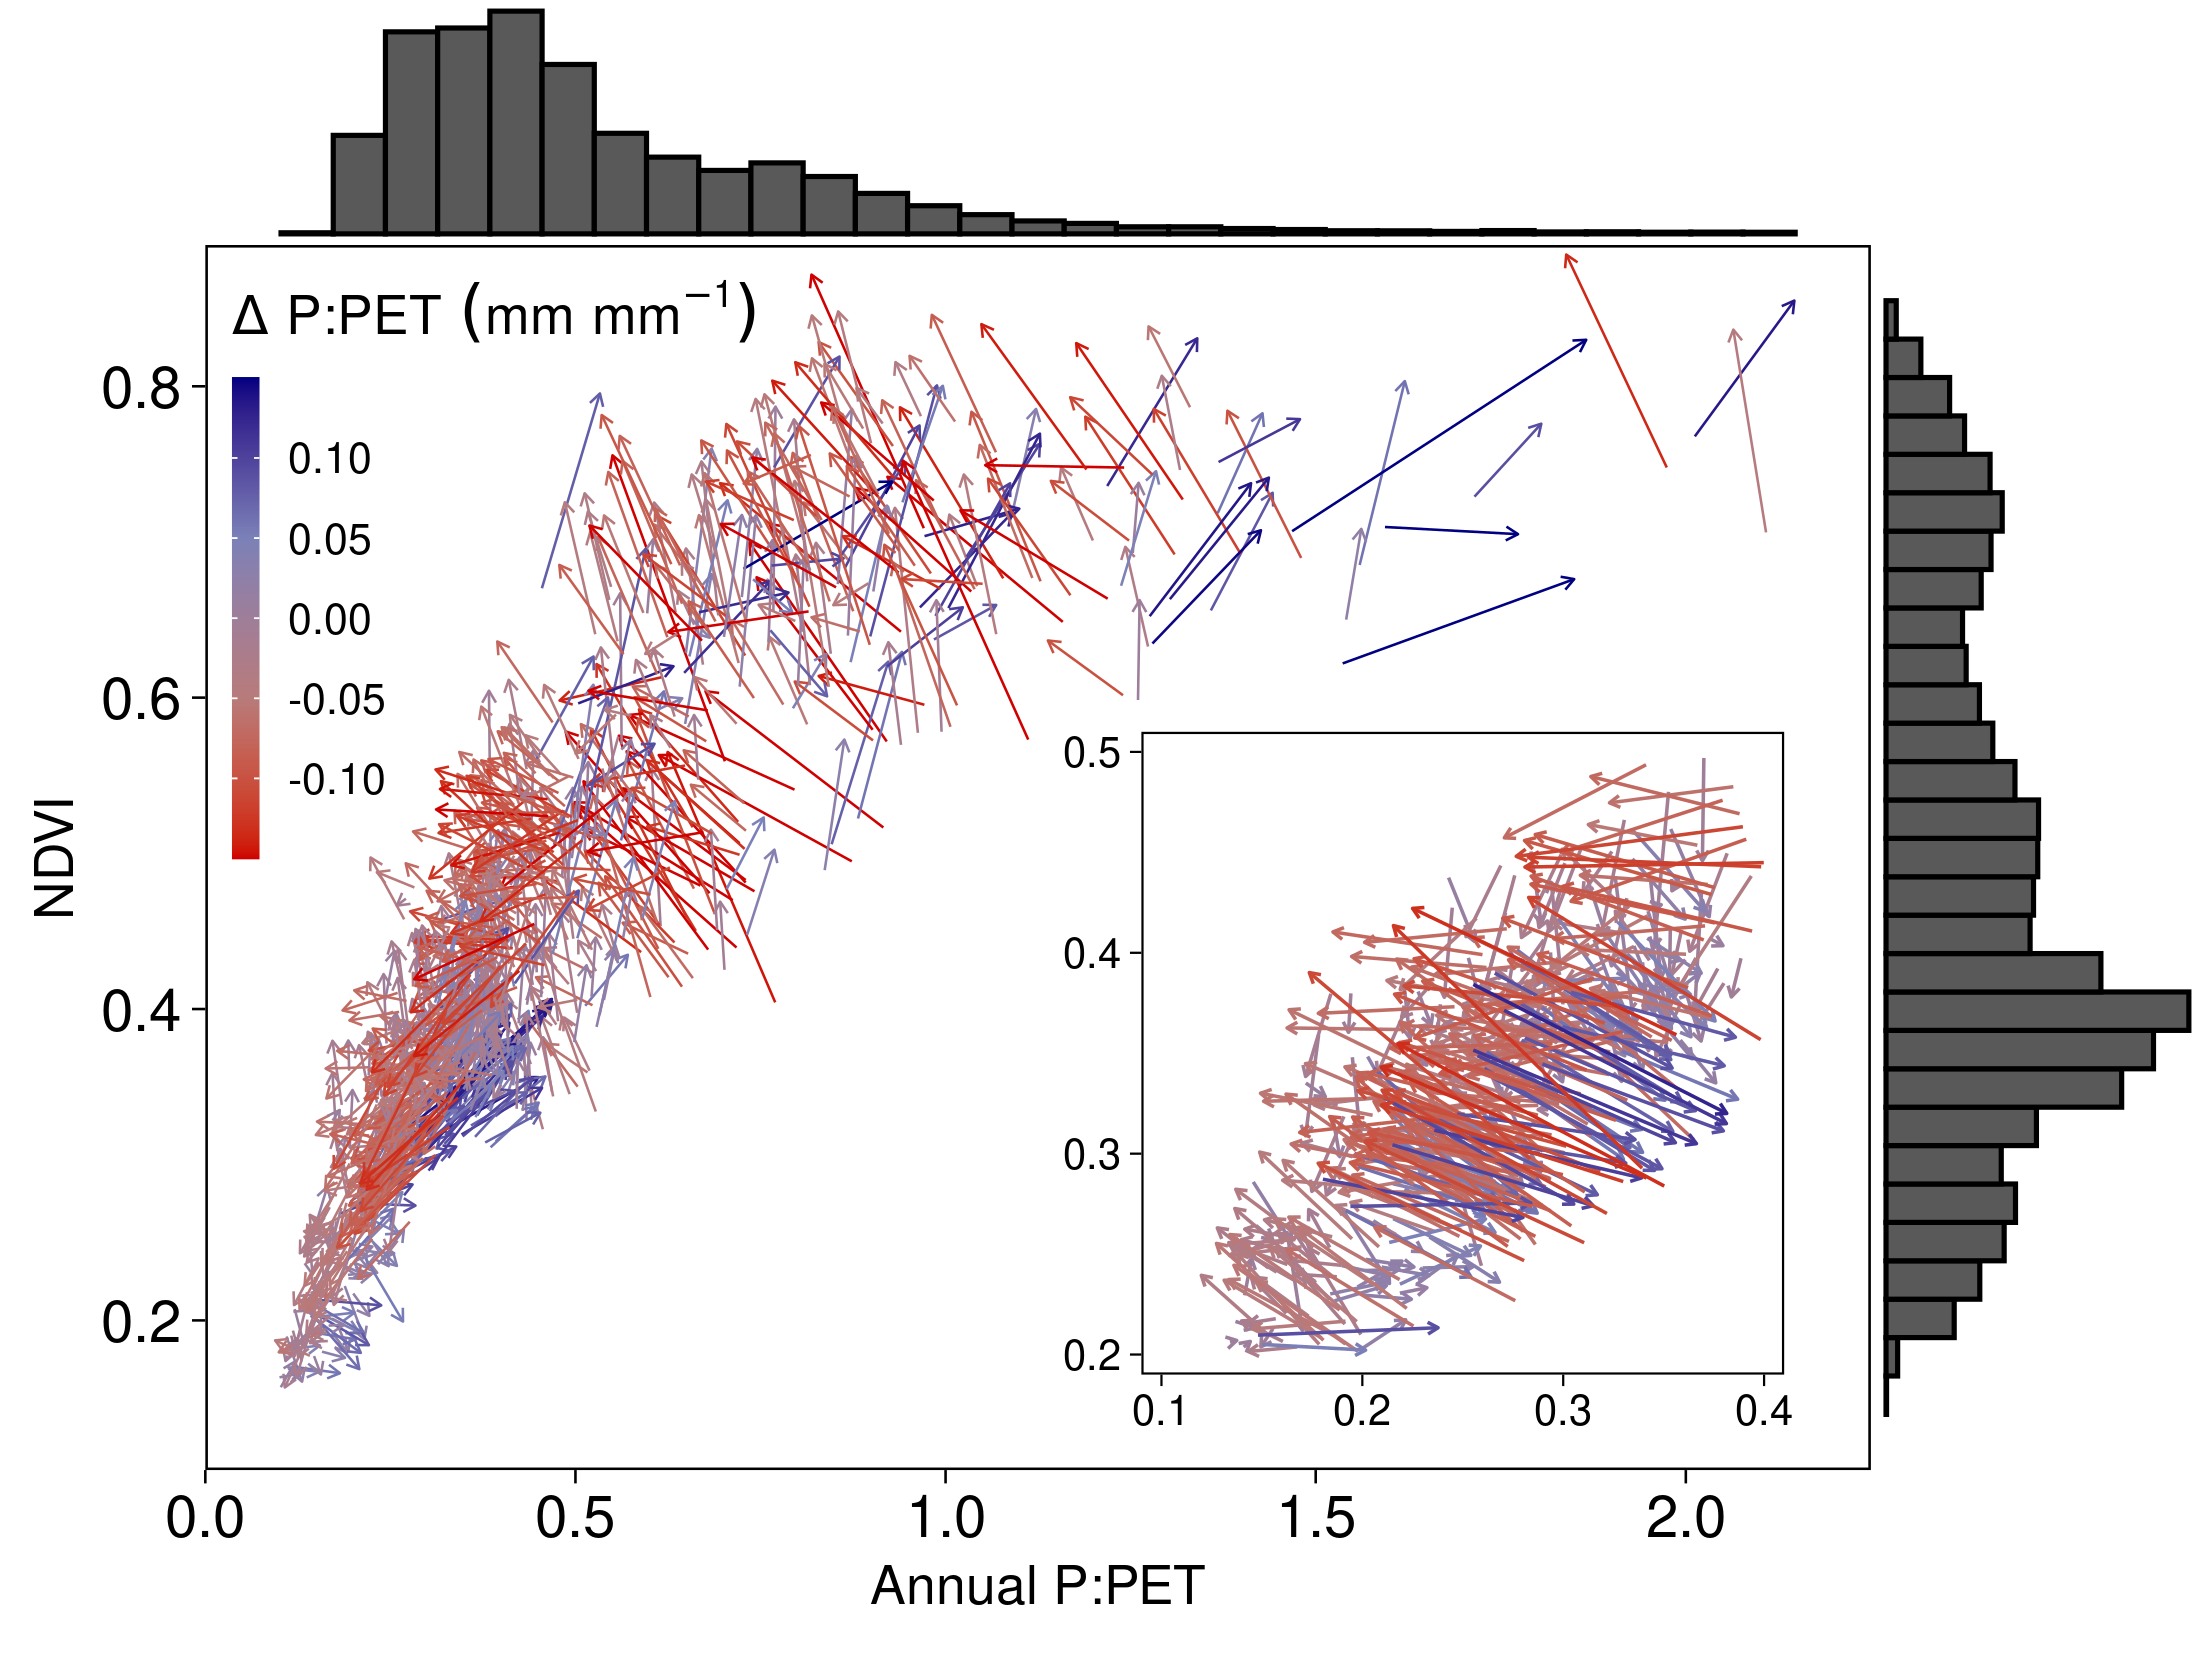
\includegraphics[width=16cm]{../../figures/Fig1_ndvi_ppet_vectorPlot_wInset} \caption{Individual grid cell temporal 38-year trajectories of the normalized difference vegetation index (NDVI) and the ratio of annual precipitation (P) to potential evapotranspiration (PET). A vector field plot showing the direction of change in mean annual NDVI and P:PET between 1982-1986 and 2015-2019 for 1000 randomly sampled grid-cell locations (color indicates direction of change in P:PET as indicated by legend). An inset shows a magnification of the samples from the 0.1-0.4 P:PET range. The distributions of mean P:PET ($mm\,mm^{-1}$) and NDVI for the period of 1982-1986 are shown as histograms above and to the right of the main panel. Note that the majority of arrows shift towards higher aridity (lower P:PET) and higher NDVI.}\label{fig:fig.align:"left"}
\end{figure}
\clearpage
\begin{figure}
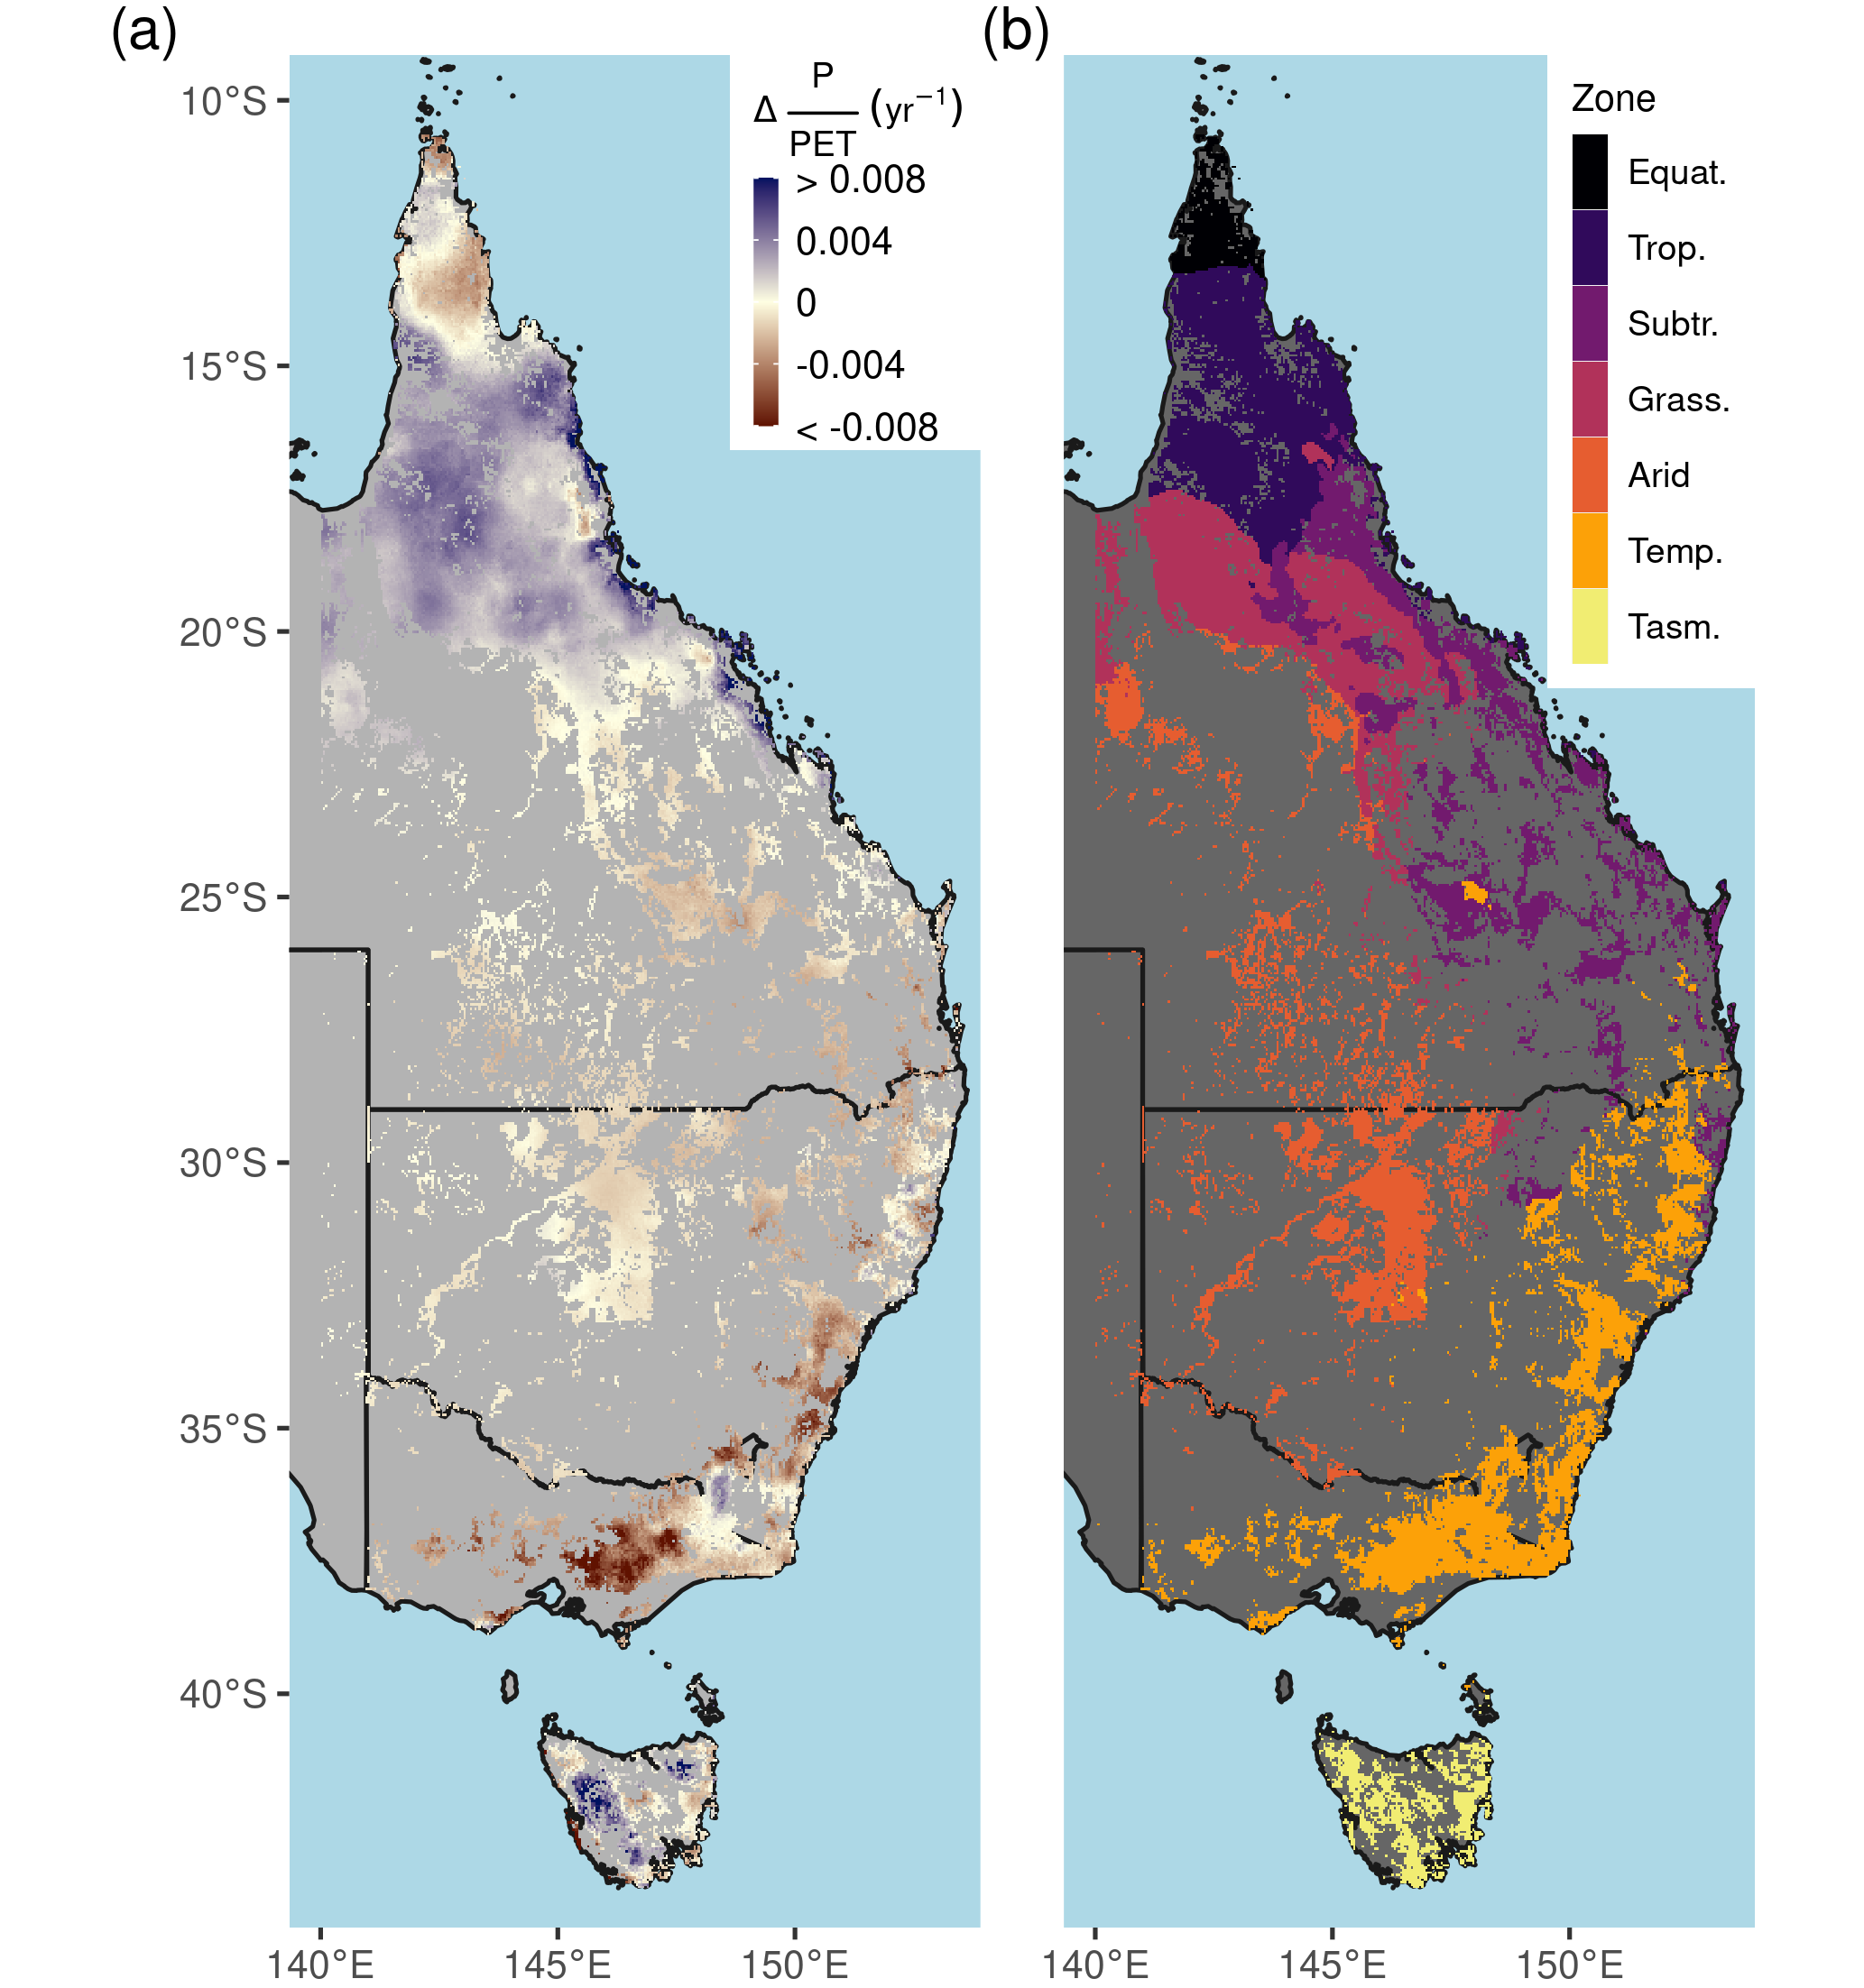
\includegraphics[width=14cm]{../../figures/Fig2_PPET-TheilSen_map-Koppen} \caption{Long-term aridity change and climate zones. (a) The linear trend of annual P:PET (the moisture index) between 1982-2019, (b) Simplified Köppen climate zones. Climate zone abbreviations correspond to Equatorial (Equat.), Tropical (Trop.), Subtropical (Subtr.), Grassland (Grass.), Temperate (Temp.), and Temperate Tasmania (Tasm.).}\label{fig:unnamed-chunk-1}
\end{figure}
\clearpage

\hypertarget{results}{%
\section{Results}\label{results}}

\hypertarget{long-term-greening-in-a-changing-climate}{%
\subsection{Long-term Greening in a changing
climate}\label{long-term-greening-in-a-changing-climate}}

Parts of northern Queensland grew wetter, but aridity (as measured by
reduced P:PET; the moisture index, MI) in over 52\% of eastern
Australian woody ecosystems since 1982 (Figs. 1,2a). Aridity decreased
over northern Queensland encompassing the entirety of Equatorial and
Tropical regions, and most of the Grassland and Subtropical regions,
driven by large wet-season increases in precipitation (Fig. A2a).
Widespread increases in PET were evident from September-February (Fig.
A2b). At the same time as these changes in climate were occurring, over
92\% of these regions experienced overall greening (Fig. 3a), including
regions where P:PET declined (Figs. 1,2b,A3). The relative increases in
NDVI were comparable between the earlier AVHRR epoch (1982-2000) and the
later MODIS epoch (2001-2019) at 5.7\% (CI={[}-2.9\%, +20.3\%{]}) and
5.1\% (CI={[}-6.4\%, +20.1\%{]}), respectively. However, the spatial
patterns of greening/browning differed between epochs (Fig. 3b), and
most regions also showed high decadal-scale variability of
greening/browning trends (Fig. 4). The overall greening trends between
the AVHRR 1982-2000 epoch and the MODIS 2001-2019 epoch generally agree
across regions and seasons. However linear NDVI trends fit over shorter
intervals of 10 years are much less consistent (Fig. 4), exemplifying
the importance of estimating trends over long enough periods to average
over decadal-scale variability. Long term browning only occurred in the
Arid region (Fig. 3,4). Nevertheless, by examining NDVI trends over
nearly forty years, we were able to separate regional decadal-scale
variability from the overall, broad greening trend across eastern
Australia (Figs. 3,4,A3).

\clearpage
\begin{figure}
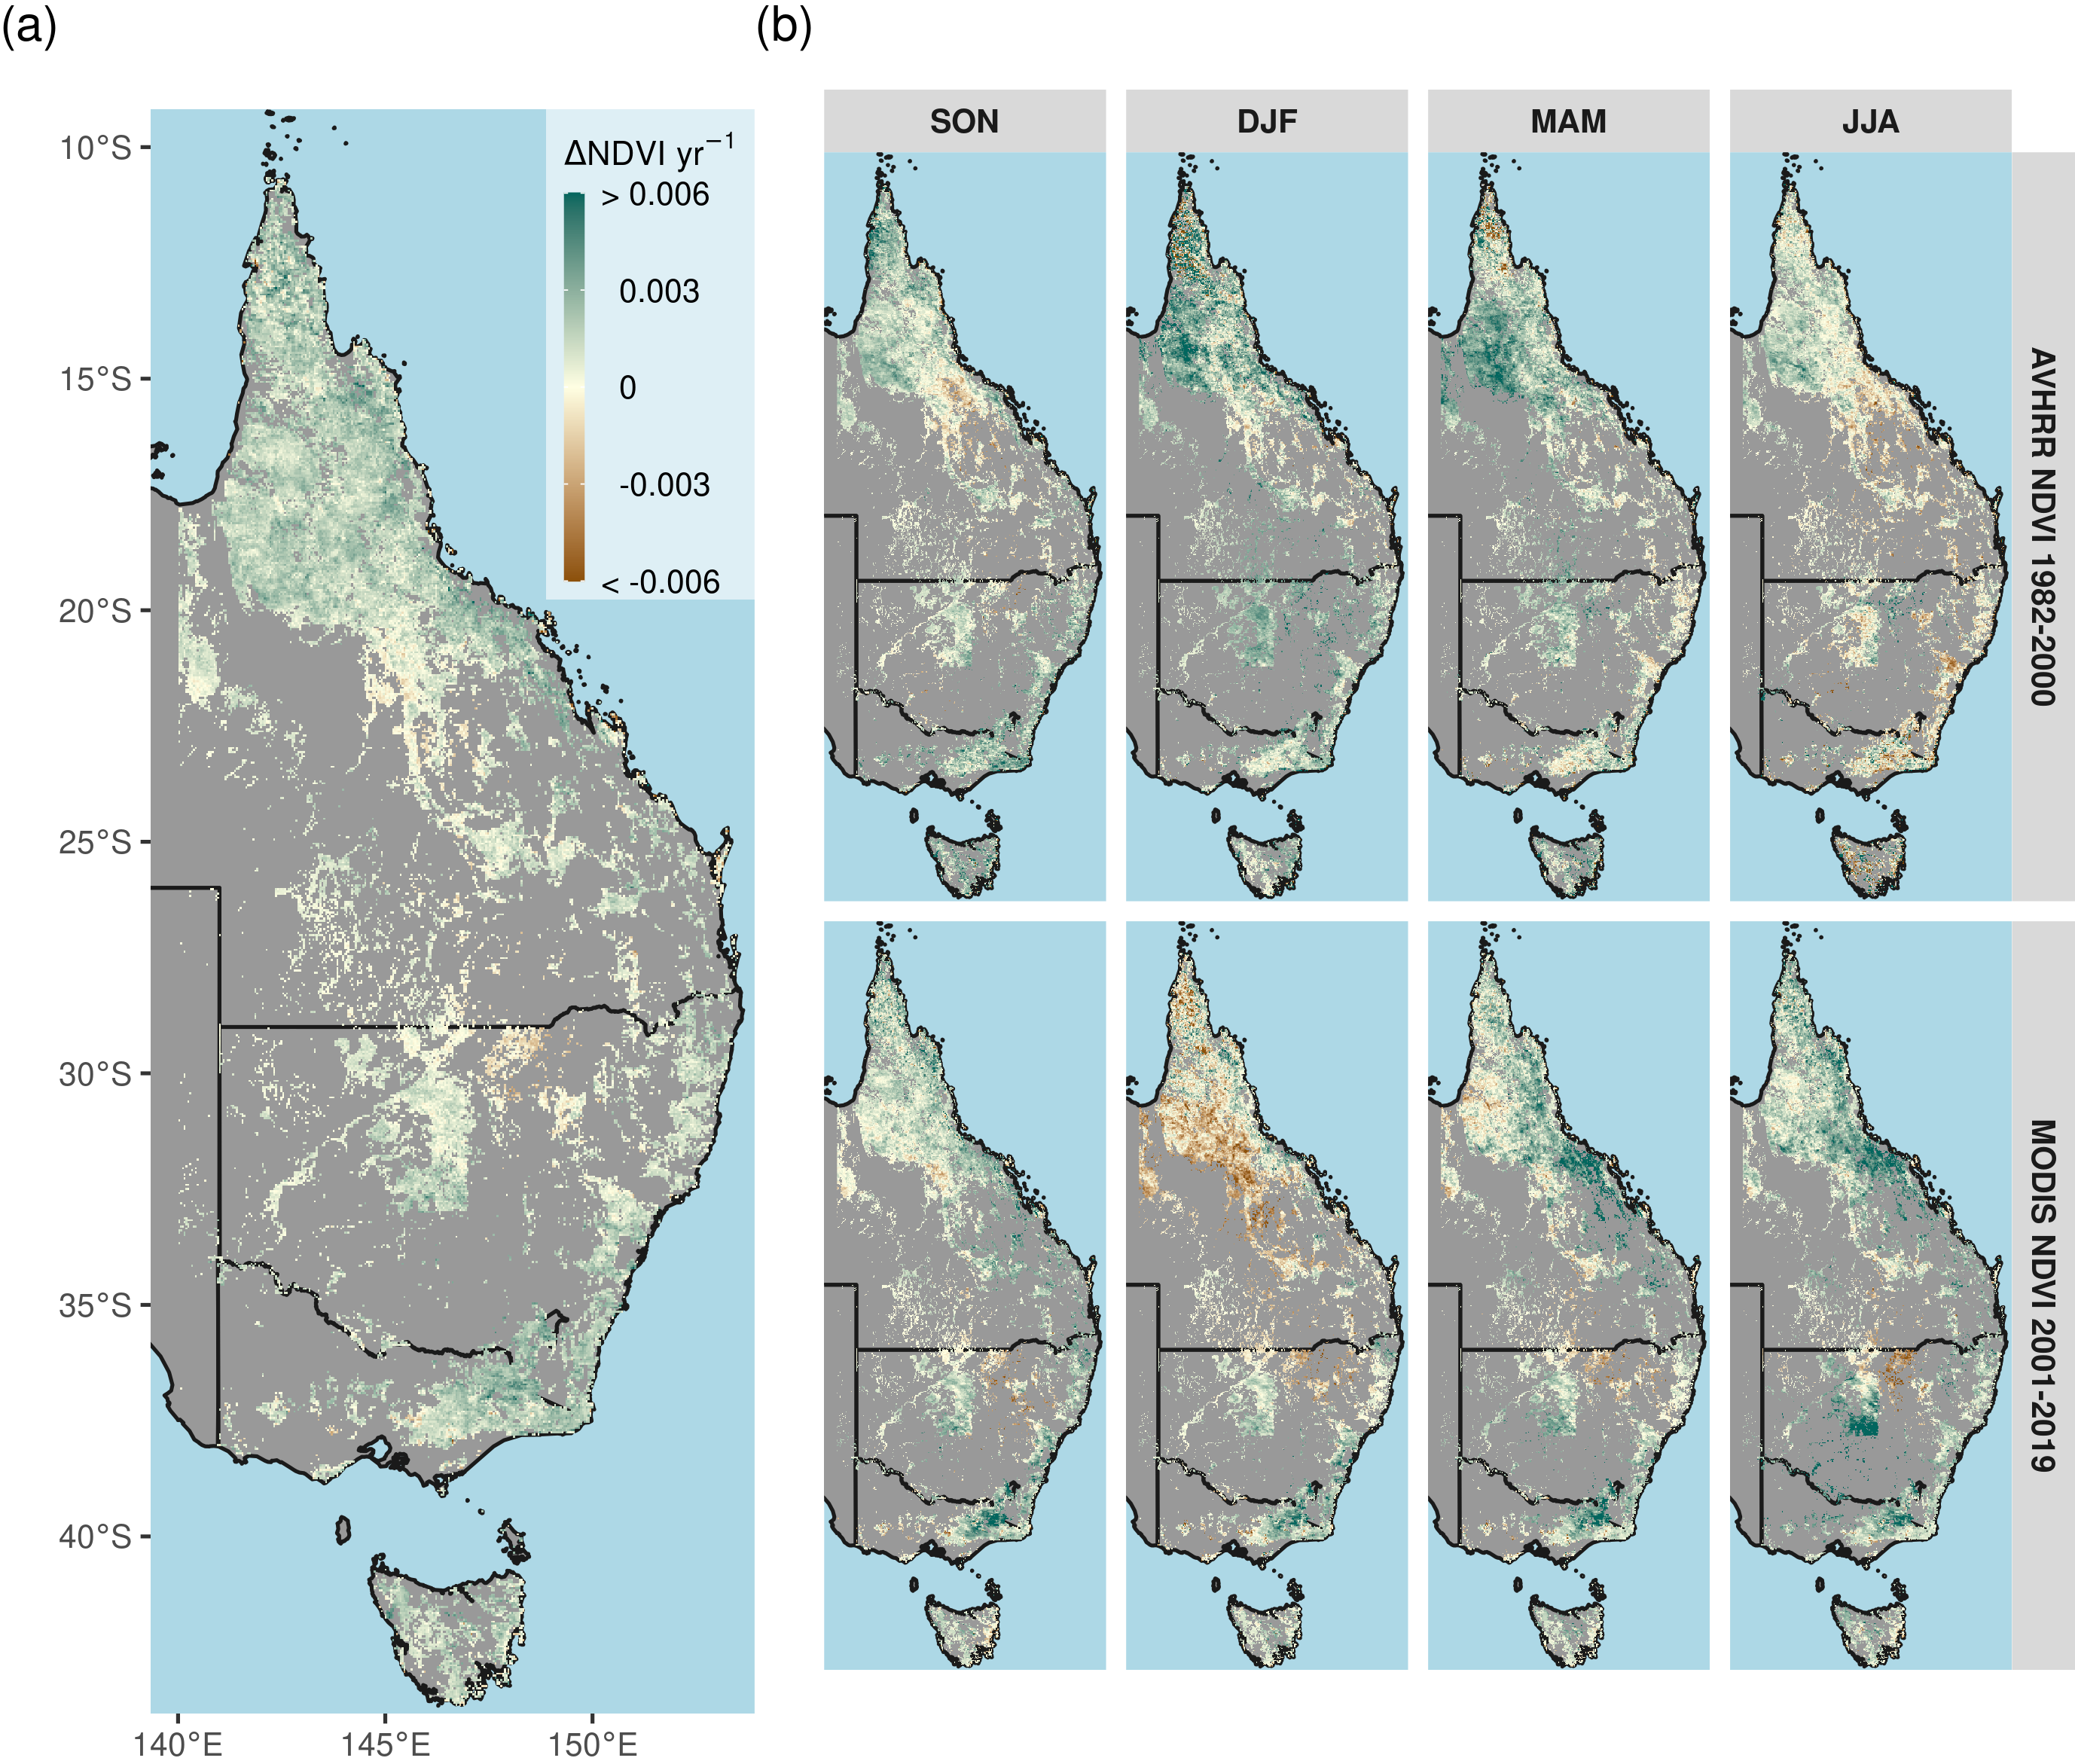
\includegraphics[width=14cm]{../../figures/Fig3_ndvi-annual-rlm_ndvi-seasonal-TheilSen-trend-by-epoch} \caption{Overall long-term NDVI change and change shown by satellite epoch and season. (a) The annual rate of NDVI change from the merged satellite record spanning 1982-2019. The seasonal AVHRR NDVI between 1982-2000 (b-top) and MODIS NDVI between 2001-2019 (b-bottom). Non woody ecosystem regions are masked in gray. A notable browning trend is evident at the interface of the Grassland and Arid regions during DJF of the MODIS time period.\linebreak Note: Season abbreviations correspond to September-October (SON), December-February (DJF), March-May (MAM), and July-August (JJA).}\label{fig:unnamed-chunk-2}
\end{figure}
\clearpage

\begin{figure}
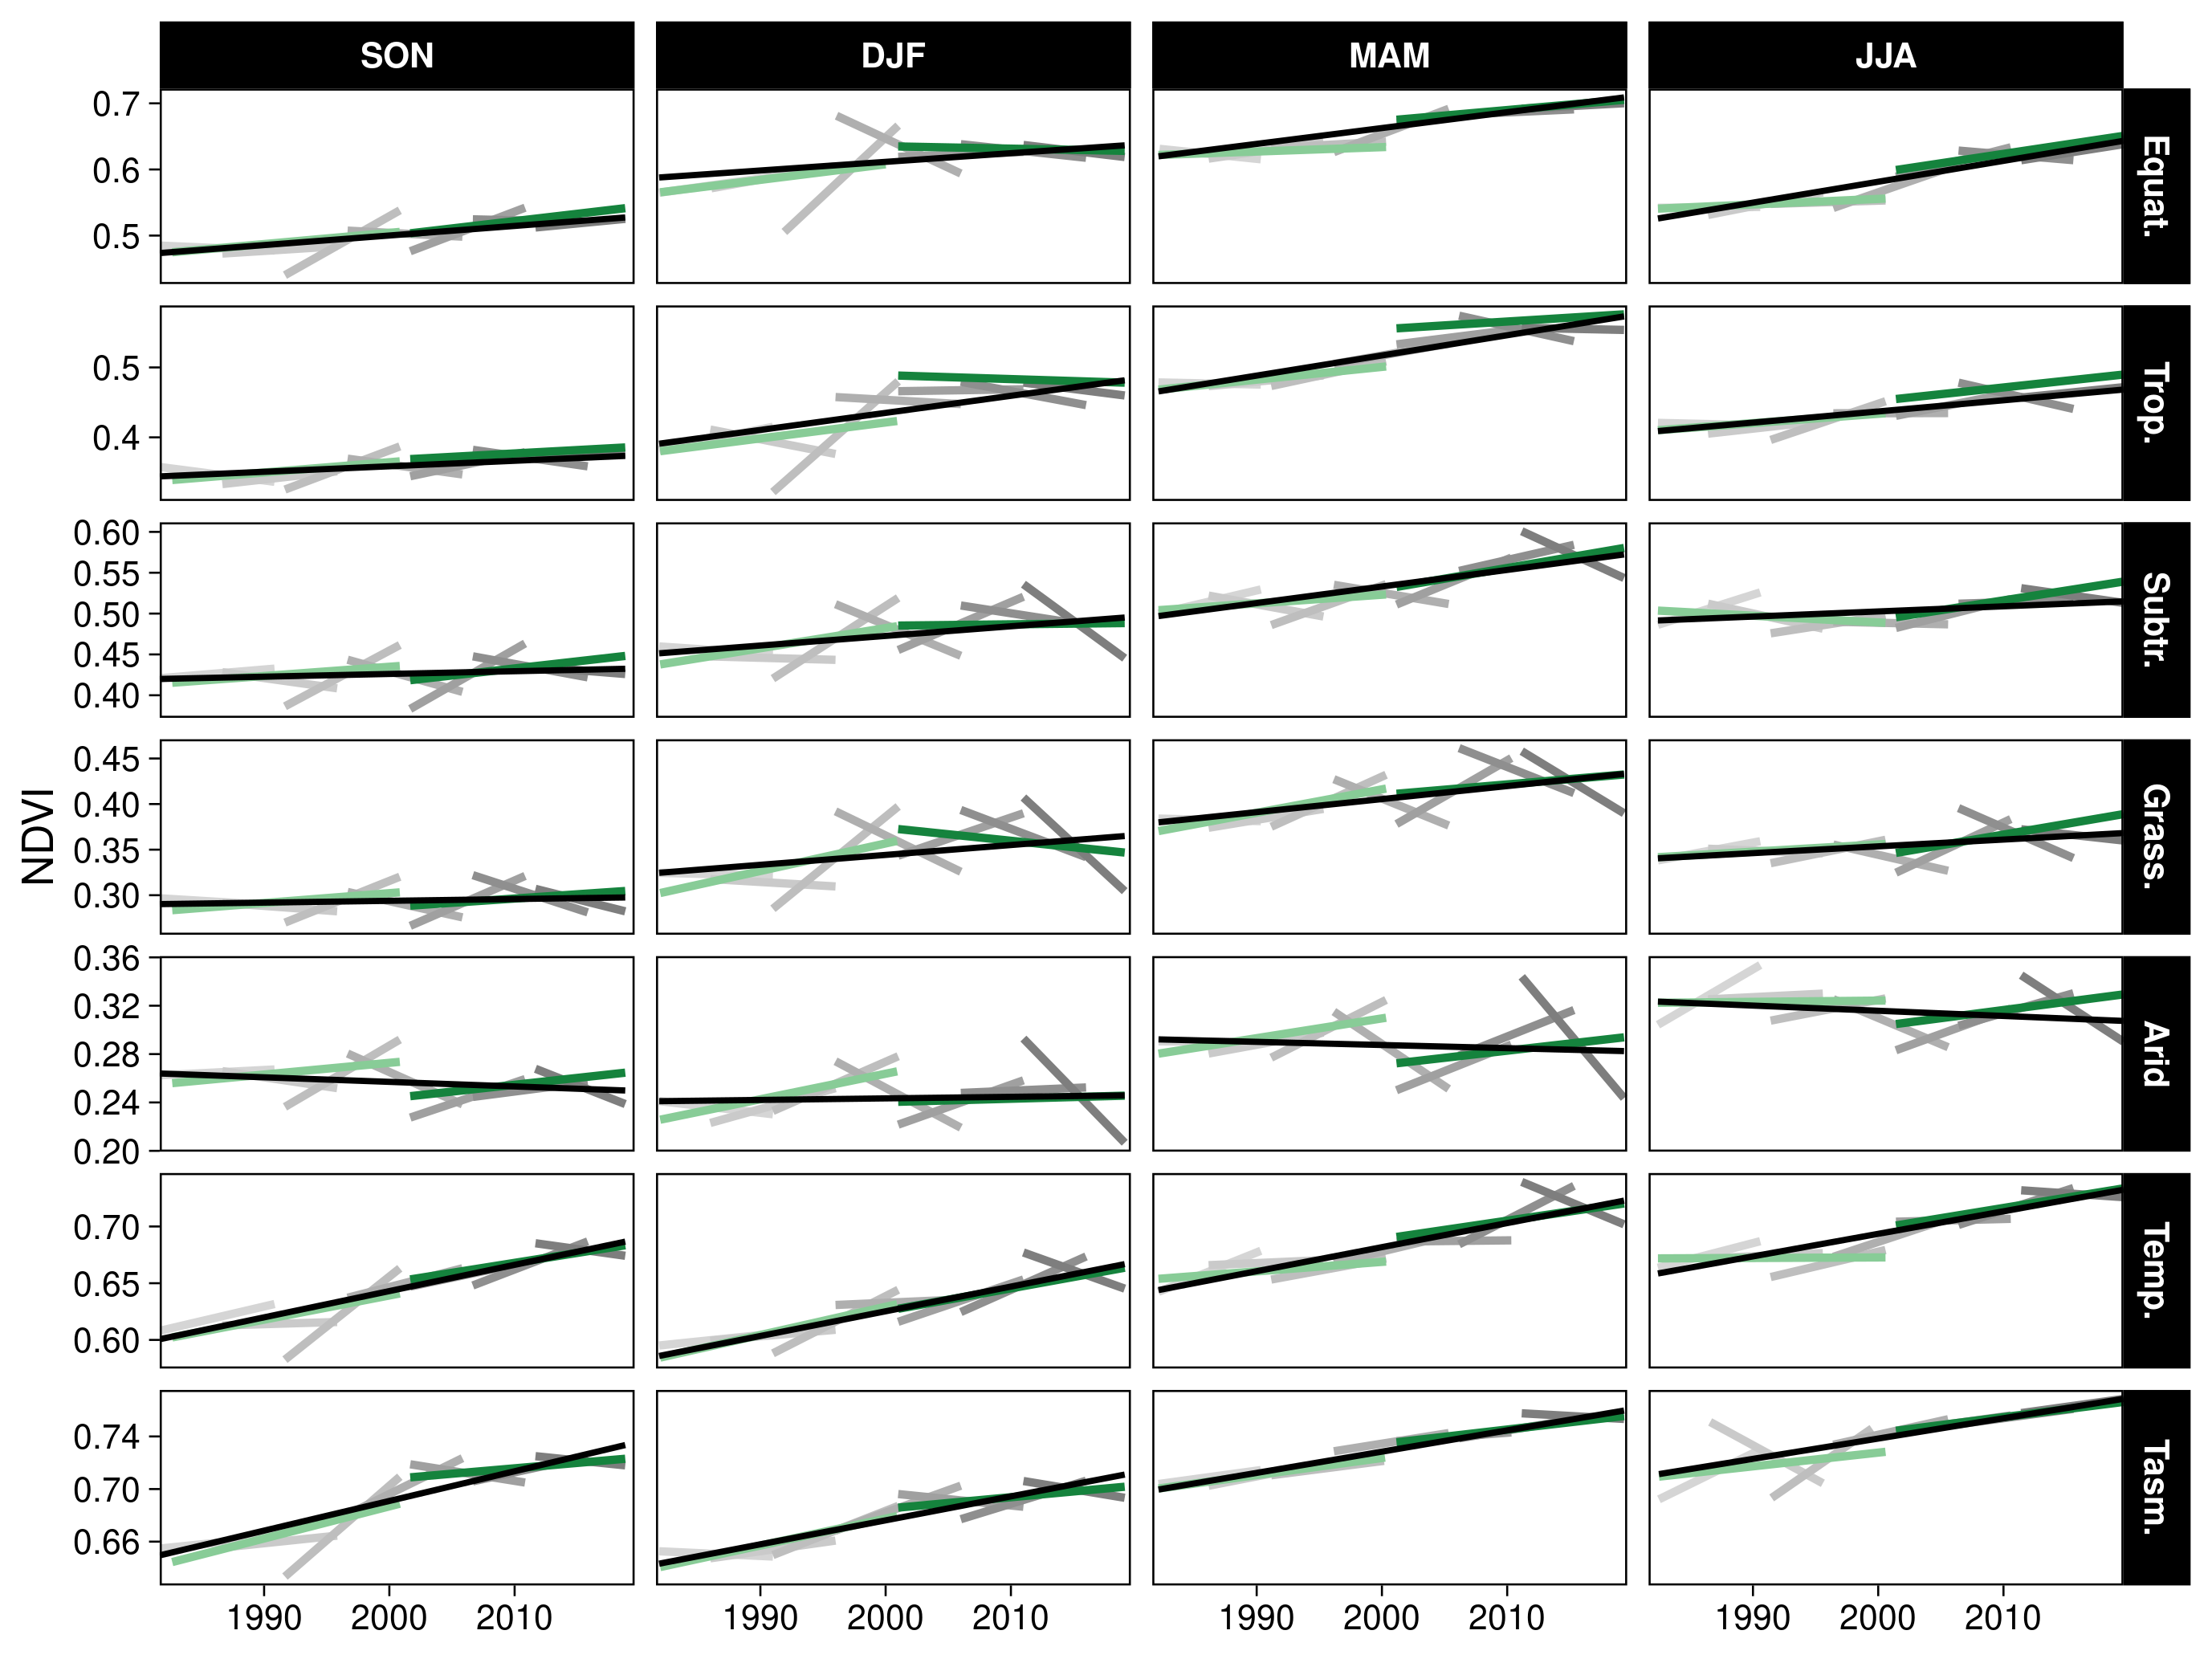
\includegraphics[width=14cm]{../../figures/Fig4_ndvi_lin_rlm_trend_10yr_segs_by_Koppen} \caption{Variability of linear trends over varying time periods by season and climate zone. The (black) line represents the overall 1982-2019 trend, the (light green) line represents the calibrated AVHRR 1982-2000, and the (green) line represents the MODIS 2001-2019. Gray colors indicate linear trends from overlapping 10 year time intervals. The boundaries of the climate zones are shown in Figure 7. \linebreak Note: Climate zone abbreviations correspond to Equatorial (Equat.), Tropical (Trop.), Subtropical (Subtr.), Grassland (Grass.), Temperate (Temp.), and Temperate Tasmania (Tasm.). Season abbreviations correspond to September-October (SON), December-February (DJF), March-May (MAM), and July-August (JJA).}\label{fig:unnamed-chunk-3}
\end{figure}
\clearpage

\hypertarget{empirical-attribution-of-the-co2-effect}{%
\subsection{\texorpdfstring{Empirical attribution of the
CO\textsubscript{2}
effect}{Empirical attribution of the CO2 effect}}\label{empirical-attribution-of-the-co2-effect}}

We found consistently positive NDVI responses to CO\textsubscript{2}
across the moisture gradient of P:PET for all seasons, with the greatest
increases located in regions of higher P:PET (\textgreater0.5) (Fig. 5).
The nonlinear Weibull models showed a larger CO\textsubscript{2}
attributable effect on NDVI in regions of higher P:PET (Fig. 5), but the
effect size of the NDVI response to CO\textsubscript{2} was largely
consistent across model forms (Figs. A4-7). The
CO\textsubscript{2}-attributable increase in NDVI between 1982-2019
ranged from approximately 5\% in the Arid interior regions to
\textgreater20\% in the wettest Tropical and Temperate regions (Fig.
5a). This was consistent with linear model forms when fit for individual
grid cell locations (equation 8; Fig. 6), as well as by comparing the
CO\textsubscript{2} effect size across 16 linear models fit for grid
cell locations grouped into bins spanning 0.1 increments of P:PET
(equation 7; Fig. A4). The GAM fit across grid cell locations also
indicated a larger CO\textsubscript{2} effect in regions with higher
P:PET (Figs. 6,7b). Quantile regression with generalized additive models
showed a pronounced response to CO\textsubscript{2} across the
distribution of pixels with both low and high NDVI (10 - 97.5
percentiles) across the full aridity gradient of P:PET (Fig. A7).\\
A recent study found the global CO\textsubscript{2} fertilization effect
was halved between the 1980s and 2000s (Wang et al. 2020). In contrast
to the estimates over eastern Australia from wangRecentGlobalDecline2020
over, we found no consistent evidence of a decline in the effect of
CO\textsubscript{2} on NDVI through time. Neither the GAM estimates nor
the robust linear model estimates of the CO\textsubscript{2} effect
showed any consistent evidence of a weakening CO\textsubscript{2} effect
between 1982-2000 and 2001-2019 (Fig. 6). The central 25-75\%
percentiles of the distribution of robust linear model effect sizes
overlapped in all regions between epochs. The central 25-75\% of the GAM
estimated distributions also overlapped, with the exception of the
Grassland and Arid regions where the CO\textsubscript{2} effect was
larger during 2001-2019. Consistent with the finding of a greater
CO\textsubscript{2} effect in wetter regions (Fig. 5), the robust linear
models and the GAM estimated the CO\textsubscript{2} effect to be
greatest in the Equatorial and Tropical regions, and lowest in the Arid
region (Fig. 6).\\
\clearpage

\begin{figure}
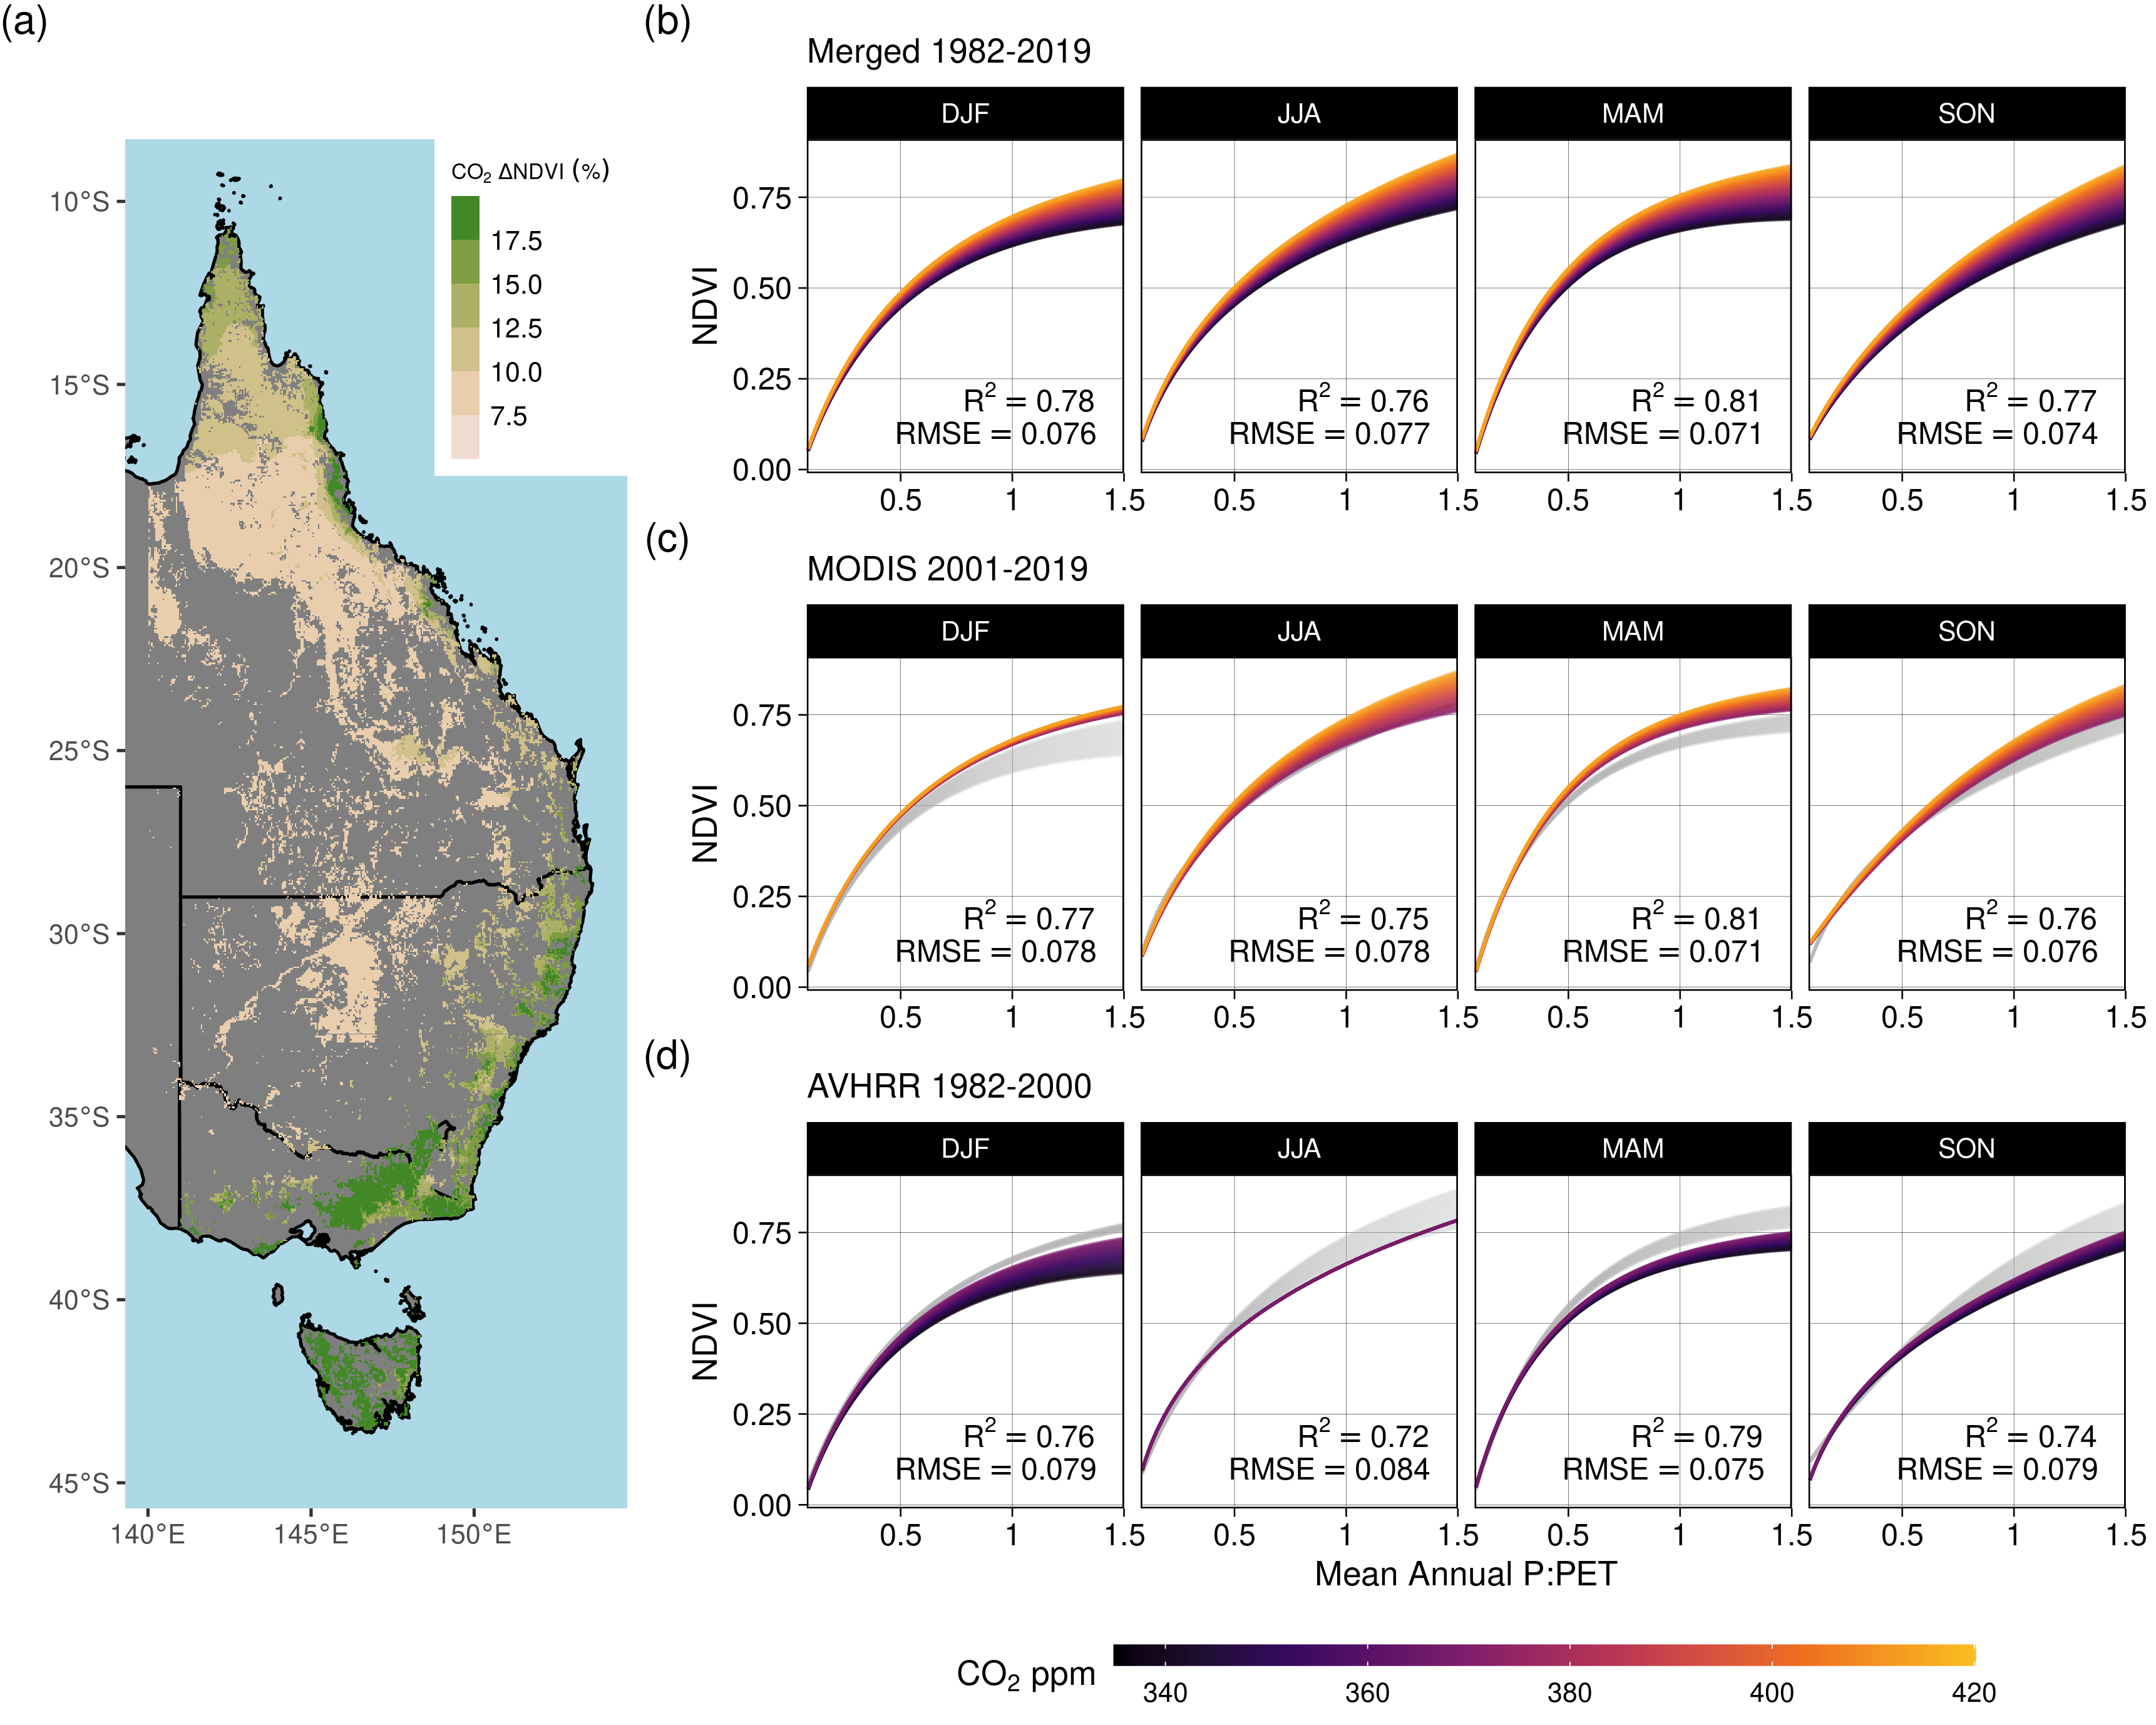
\includegraphics[width=14cm]{../../figures/Fig5_n4_ndvi_map_weibull_ppet_x_co2_modeled_effect} \caption{Effect of increasing $CO_2$ on seasonal NDVI across P:PET. Predictions of seasonal NDVI as a function of mean annual P:PET fit using a standard Weibull function (methods - eq 2), modified with linear effects of $CO_2$, the running 12-month anomaly of P:PET, and the satellite sensor. The $CO_2$ concentration gradient represents the atmospheric $CO_2$ change between 1982-2019. Panel (a) maps the total predicted contribution of $CO_2$ towards the relative increase of NDVI between 1982-2019 assuming no anomaly of P:PET. Panel (b) shows the merged sensor response between 1982-2019 across the gradient of P:PET, (c) shows the model response when fit using just MODIS MCD43 data between 2001-2019, and (d) shows the response when the model was fit with the recalibrated AVHRR data between 1982-2000. The AVHRR and MODIS satellite epoch NDVI predictions are plotted in gray for panels B and C, respectively.}\label{fig:unnamed-chunk-4}
\end{figure}
\clearpage

\clearpage
\begin{figure}
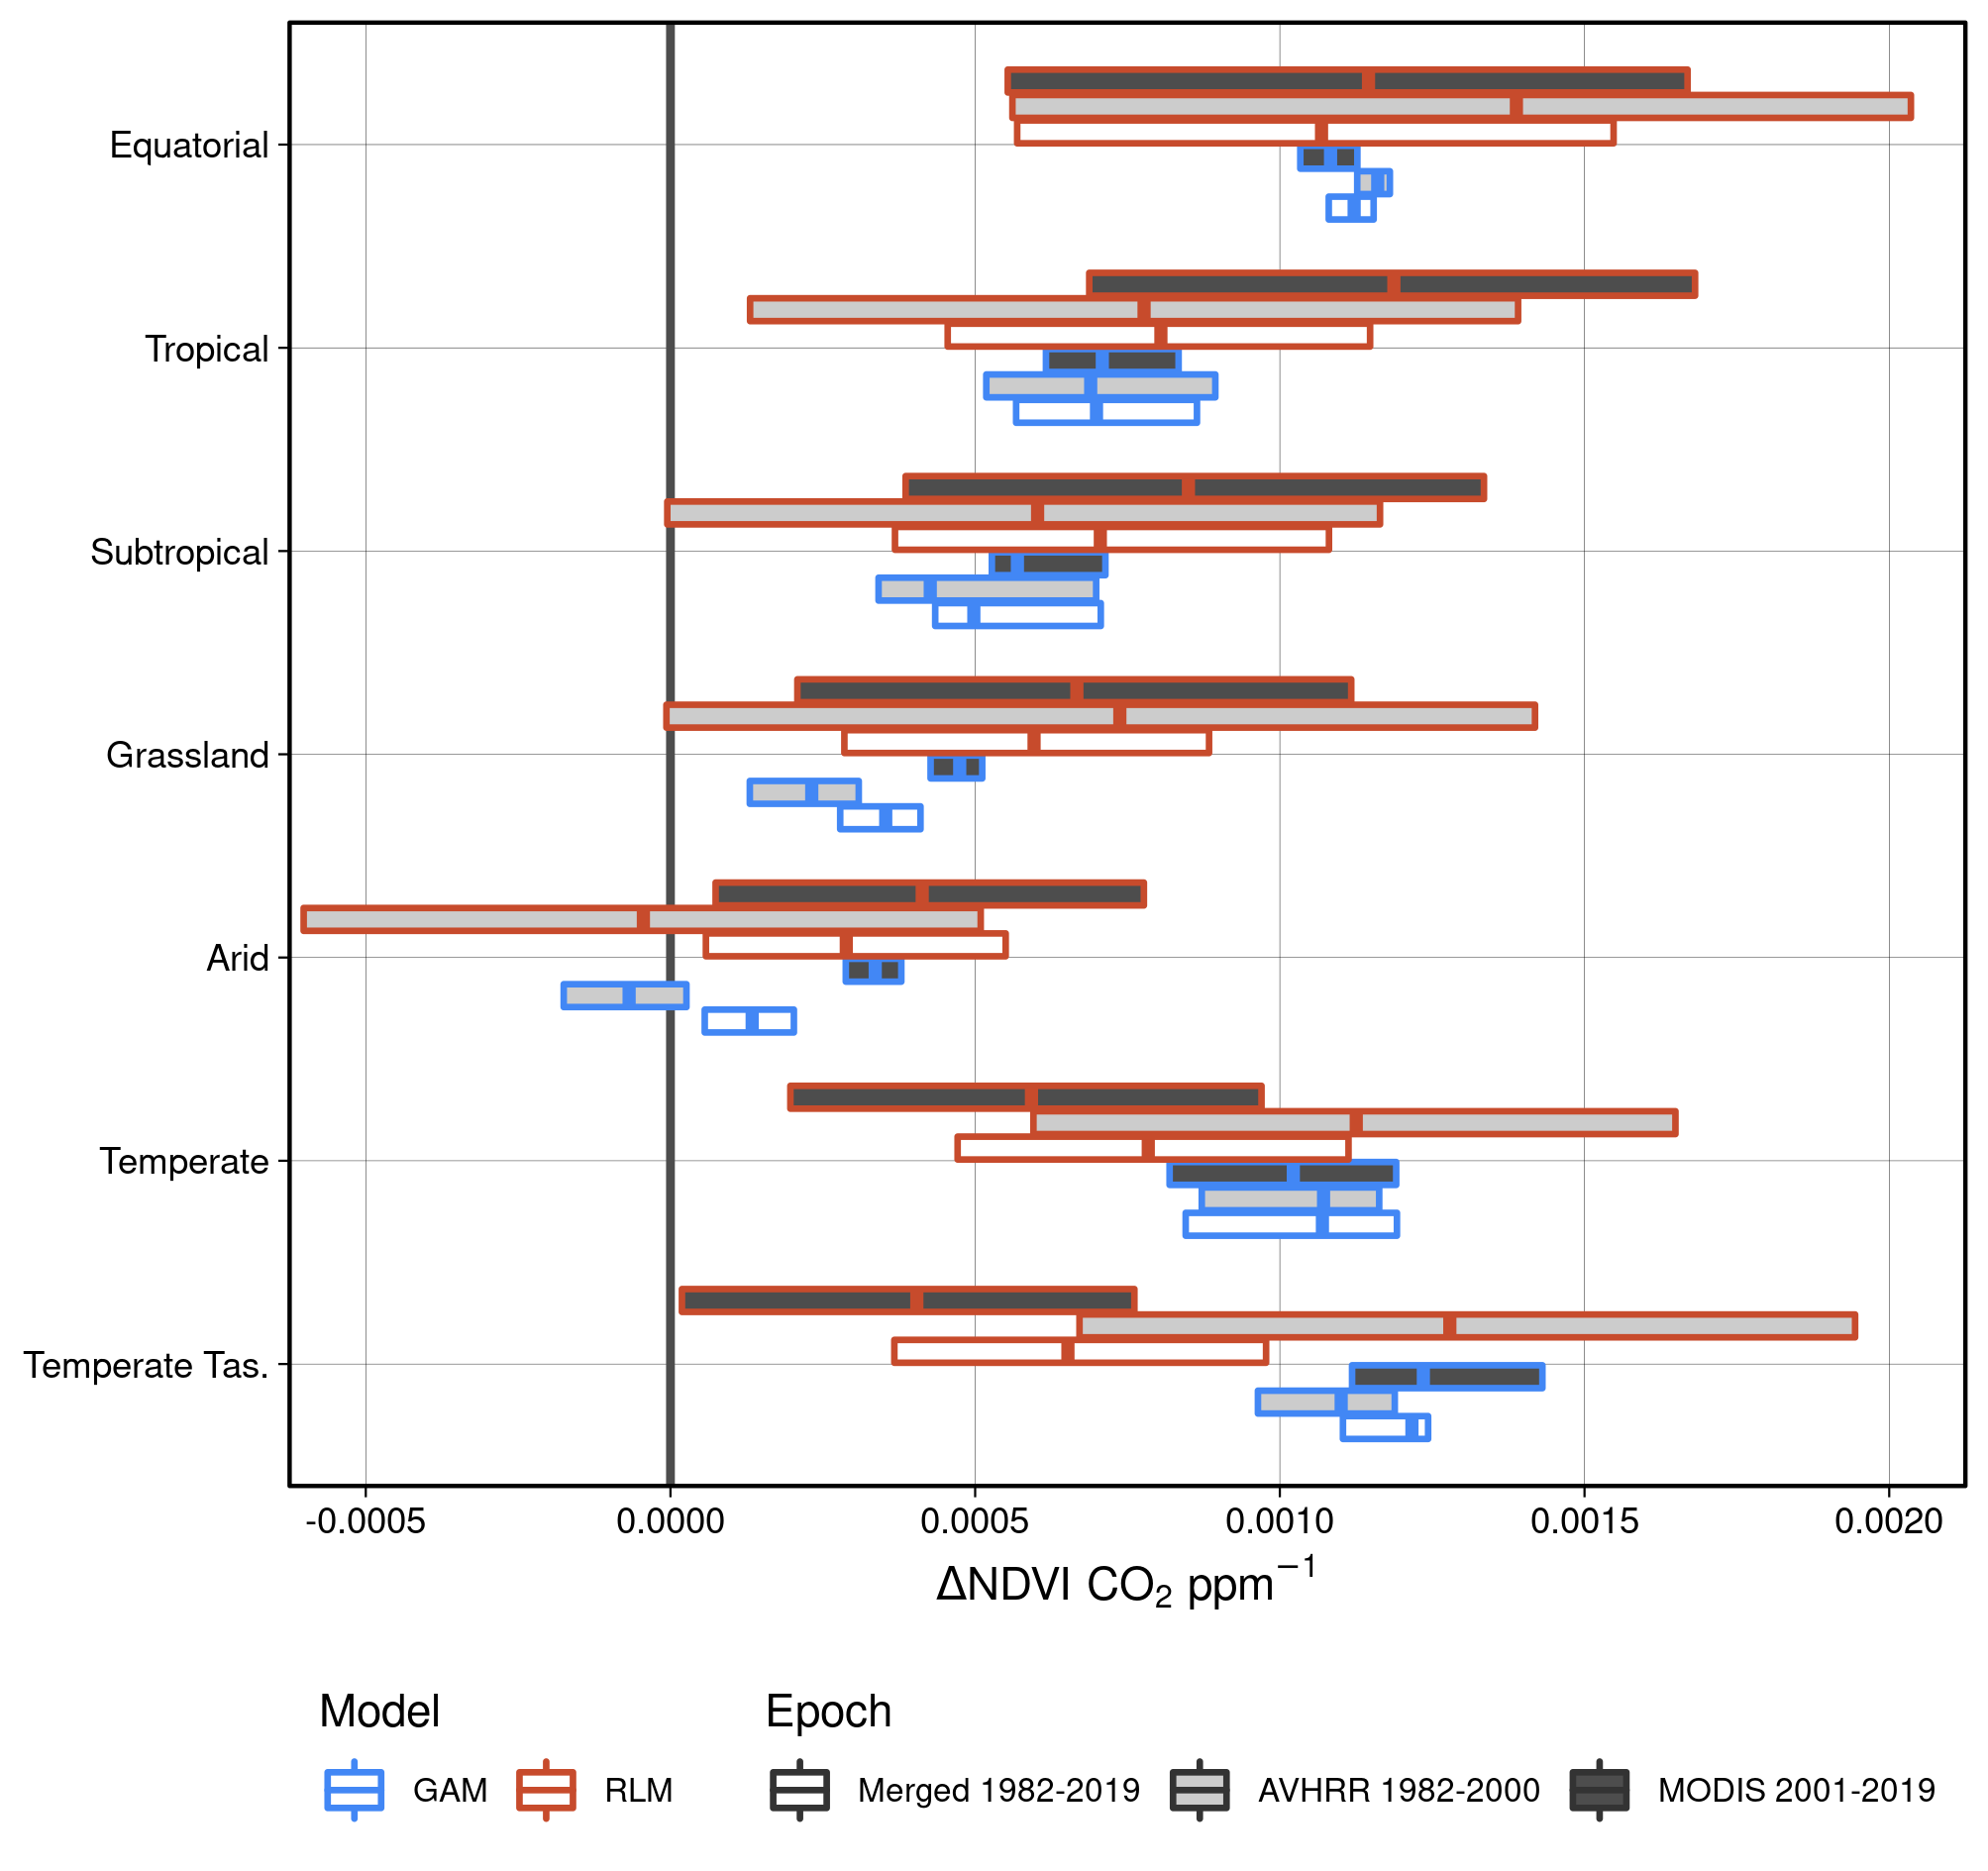
\includegraphics[width=14cm]{../../figures/Fig6_rlm_CO2_effect_by_epoch} \caption{Boxplot representation of the $CO_2$ attributable effect upon changing NDVI. Here the 25th, 50th, and 75th percentiles of the $CO_2$ attributable effect on NDVI are shown. The robust linear models (RLM; methods - eq 13) were fit for each individual grid cell location, whereas the generalized additive model (GAM; methods - eq 14) was fit using all grid cell locations. The distribution of RLMs yielded a median $R^2$ of 0.58 and RMSE of 0.025 over the merged period. The GAM had an overall $R^2$ of 0.91 and RMSE of 0.049.}\label{fig:unnamed-chunk-5}
\end{figure}
\clearpage

\hypertarget{co2-driven-greening-and-expectations-from-water-use-efficiency}{%
\subsection{\texorpdfstring{CO\textsubscript{2} driven greening and
expectations from water use
efficiency}{CO2 driven greening and expectations from water use efficiency}}\label{co2-driven-greening-and-expectations-from-water-use-efficiency}}

The range of statistically estimated CO\textsubscript{2}-attributable
greening responses was compared with the expectation from the
theoretical CO\textsubscript{2} water use efficiency model. The Donohue
et al.~(2013) CO\textsubscript{2} x WUE model (see methods) accounts for
changes in VPD, but assumes no change in water supply. Assuming an equal
split in the benefits of WUE between greater carbon assimilation and
increased foliage cover (see below for alternative assumptions), the
model predicted an 8.7\% (10-90\% percentile range {[}+6.8\%,+10.2\%{]})
increase in NDVI (proxy for foliage cover, see methods). This compared
to an estimated 11.7\% ({[}+4.6\%,+14.6\%{]}) relative increase from the
GAM, when accounting for simultaneous increase in VPD (which the WUE
accounts for), and factoring out the effects of changing precipitation
and PET (which the WUE model does not account for). We needed to assume
differing levels of allocation to foliar gain (i.e.~not 50\%) for the
theoretical WUE model to match the statistically estimated
CO\textsubscript{2} effect (Fig. 7d). Regions of higher P:PET
(Equatorial, Tropical, Temperate, and Temperate Tasmanian) required
greater allocation fractions than 50\%, whereas the allocation fraction
would be between 25-50\% for regions with lower P:PET (Arid, Grassland,
and Subtropical). In comparison, the PETA hypothesis (Donohue et al.
2017) predicted the greatest CO\textsubscript{2} effect on leaf area to
be in regions with the lowest LAI, but this was not supported by the
statistically estimated CO\textsubscript{2} effect on NDVI (Fig. A9).
Despite having the lowest LAI, the Arid region received the smallest
CO\textsubscript{2} effect, but it is worth noting the Arid region also
experienced the greatest increase in VPD and reduction in P over the 38
year period (Fig. 7a, A8). In contrast, the largest estimated
CO\textsubscript{2}-attributable effect on greening were found to be in
the Equatorial and Tropical areas.

\hypertarget{co-occurring-shifts-in-aridity-ndvi-and-vegetation-cover}{%
\subsection{Co-occurring shifts in aridity, NDVI, and vegetation
cover}\label{co-occurring-shifts-in-aridity-ndvi-and-vegetation-cover}}

The shifts in P:PET and NDVI were accompanied by vegetation cover
changes in some regions. Most notably, the Arid and Temperate regions
experienced the strongest zonally averaged declines in P:PET (Fig. 8a)
and increases in VPD (Fig. A8). Seasonal greening trends were relatively
similar apart from the aforementioned exceptions in the Grassland. The
MODIS vegetation continuous fraction data from 2001-2018 indicated most
regions experienced modest changes in tree vegetation cover. The largest
decline in tree cover occurred in the Temperate regions (Fig. 8c,A10.
Most regions experienced declines in non-vegetated (bare) cover,
increases in non-tree vegetation, and modest change in tree-cover (Fig.
8c), however the proportional increase of non-tree vegetation typically
exceeded tree cover increases (Fig. A10).

\clearpage
\begin{figure}
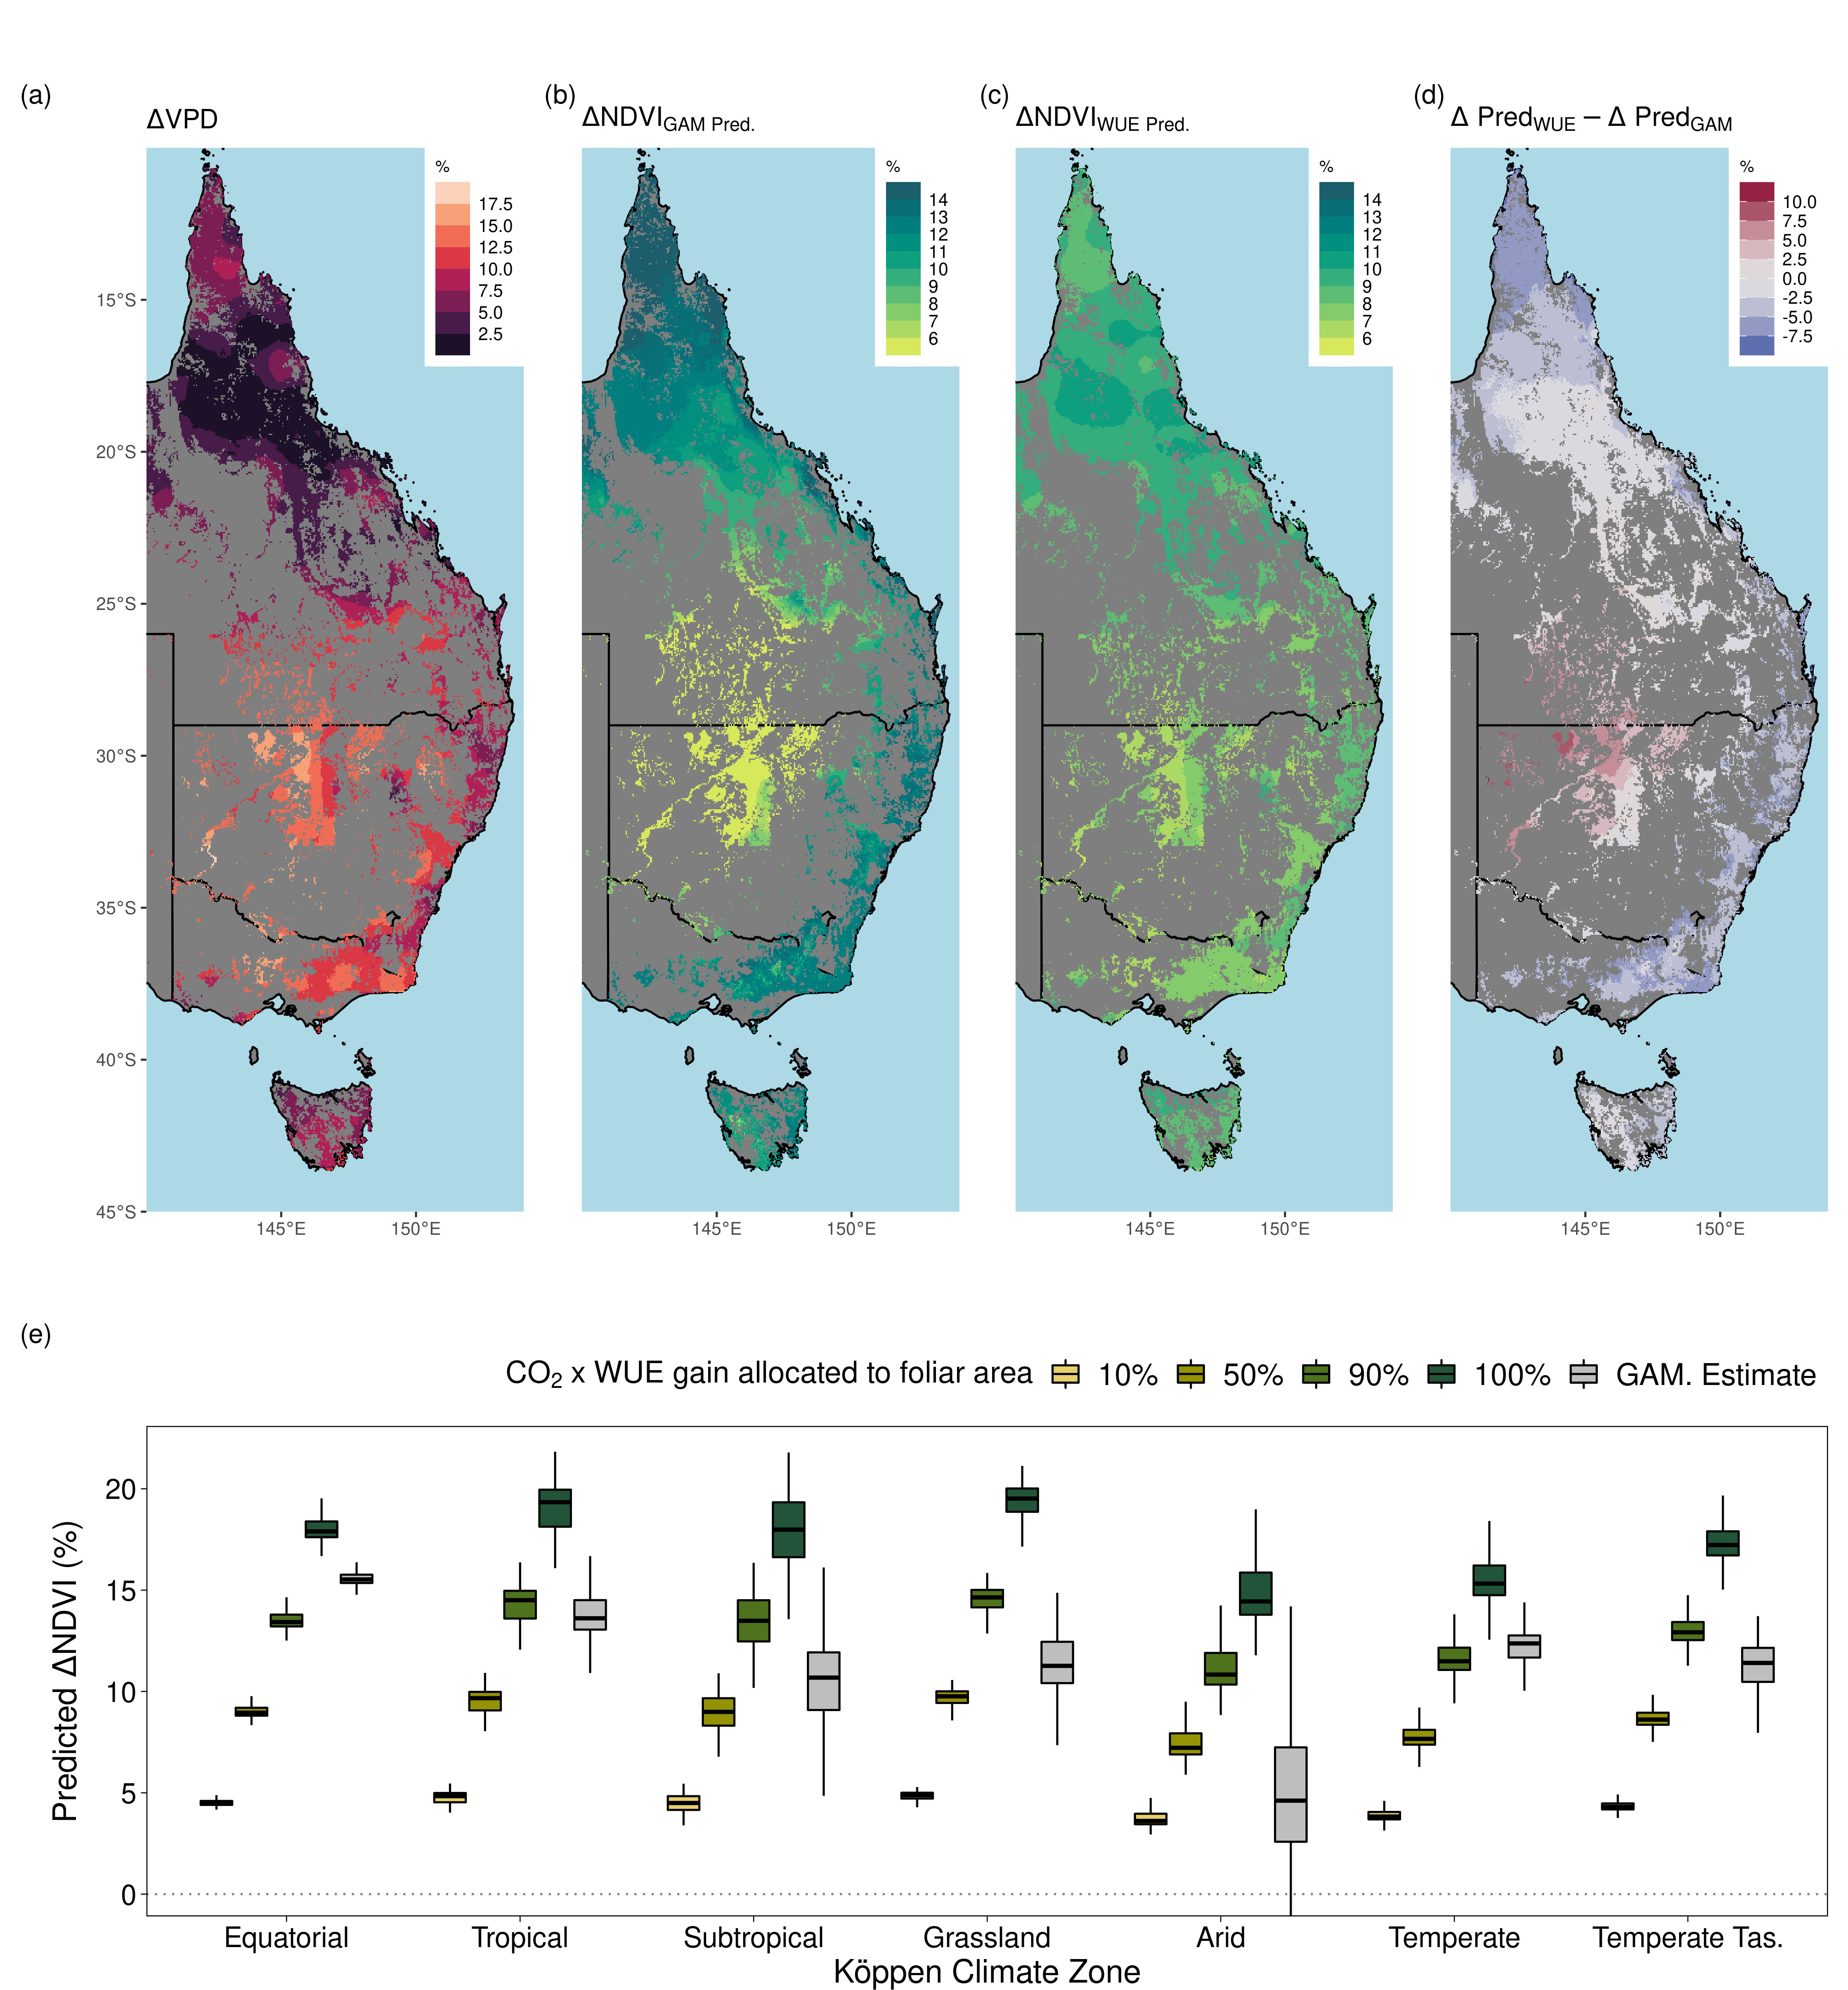
\includegraphics[width=14cm]{../../figures/Fig7_map_dVpd_gamCO2Pred_wueCO2Pred_dDifferenceBoxplot} \caption{Long-term changes in vapor pressure deficit, and comparison between the $\Delta~NDVI$ due to $CO_2$ and the expected $CO_2$ fertilization effect on foliar area due to gains in water use efficiency (WUE). (a) The relative increase in the annual mean of vapor pressure deficit (VPD) between 1982-2019. (b) The predicted relative increase in NDVI due to $CO_2$ (methods - eq 14) with a concurrent increase in VPD. (c) The relative expected increase in NDVI following the theoretical WUE prediction where 50\% of the gain is allocated to foliar area (methods - eq 11).}\label{fig:unnamed-chunk-6}
\end{figure}
\clearpage

\clearpage 
\begin{figure}
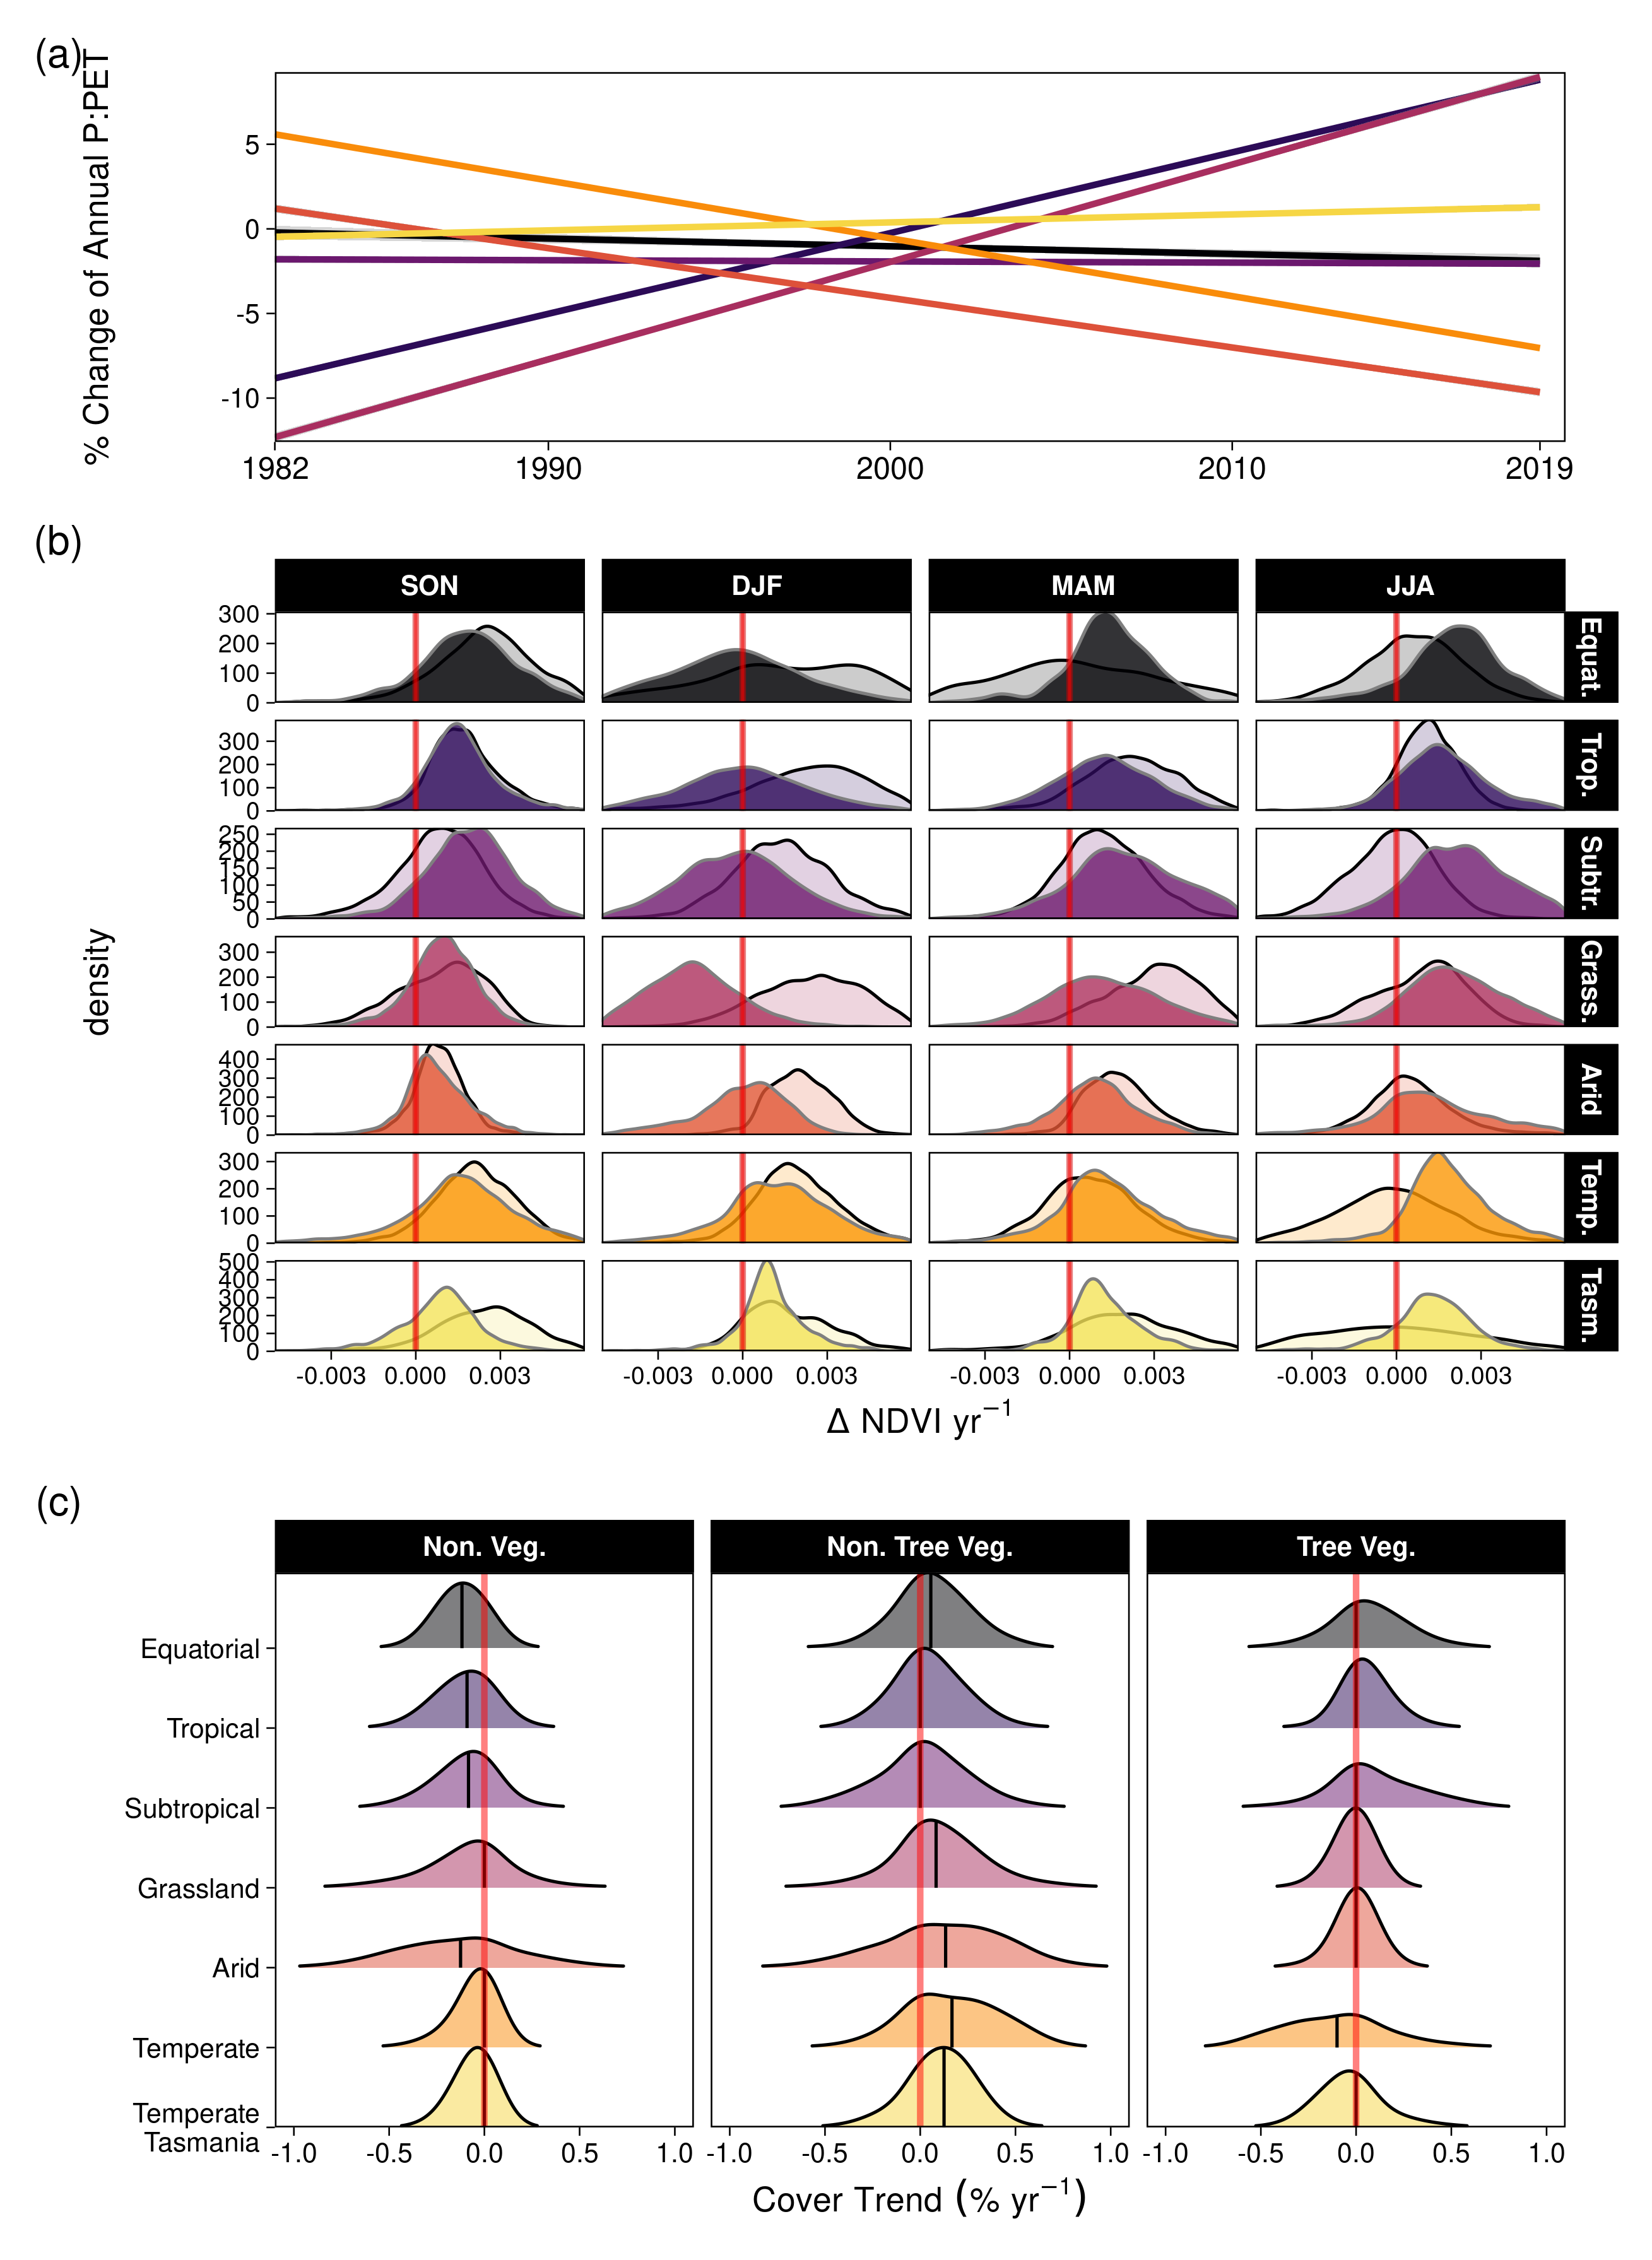
\includegraphics[width=12cm]{../../figures/Fig8_PPET_change_ThielSen_VCF} \caption{The relative percentage change in P:PET by climate zone and corresponding distributions of $\Delta~NDVI~yr^-1$ and percentage annual change in vegetation cover fraction. (a) The linear relative changes in annual P:PET trend by climate zone between 1982-2019, as estimated by robust regression (methods). (b) Distribution of linear long term NDVI trends for the six climate clusters by season using the Theil-Sen estimator. Filled distributions are trends from the MODIS sensors (2001-2019) and transparent (black outline) distributions are from the AVHRR sensors (1982-2000). (c) Distributions of the linear pixel level trends using the Theil-Sen estimator for non-vegetated cover, non-tree vegetation cover, and tree cover between 2000-2018. The 25, 50, and 75\% quantiles are overlaid. \newline Note: Climate zone abbreviations are as follows: Equatorial (Equat.), Tropical (Trop.), Subtropical (Subtr.), Grassland (Grass.), Temperate (Temp.), and Temperate Tasmania (Tasm.).}\label{fig:unnamed-chunk-7}
\end{figure}
\clearpage

\hypertarget{discussion}{%
\section{Discussion}\label{discussion}}

\hypertarget{australian-woody-vegetation-as-model-systems-to-quantify-co2-fertilization}{%
\subsection{\texorpdfstring{Australian woody vegetation as model systems
to quantify CO\textsubscript{2}
fertilization}{Australian woody vegetation as model systems to quantify CO2 fertilization}}\label{australian-woody-vegetation-as-model-systems-to-quantify-co2-fertilization}}

Australia is ideal to explore the CO\textsubscript{2} contribution
towards vegetation greening because there are fewer confounding effects
to drive greening. Forest trees are evergreen and the growing season is
rarely limited by temperature or radiation. The study region spans a
large moisture gradient (Fig. A1a), but unlike much of the global
tropics, the large majority of the study region is not so cloudy as to
prevent multiple high quality multispectral satellite retrievals per
month. Australia has also not been subjected to other prominent drivers
of greening such as nitrogen deposition (Ackerman, Millet, and Chen
2019). Nevertheless, Australia has experienced notable land-use change
during the study period such as high rates of deforestation in
Queensland and northern New South Wales (Evans 2016). However, we
excluded affected pixel locations from the analysis.

Prior global analyses on warm arid environments have quantified the
CO\textsubscript{2} effect on greening (Donohue et al. 2013), yet a more
expansive global-scale analysis of all terrestrial vegetation using
dynamic global vegetation model attribution did not connect Australia's
greening to changes in atmospheric CO\textsubscript{2} concentration
(Zhu et al. 2016). Australian studies documented the greening trend up
to 2010 using the long-term AVHRR record (Donohue, McVICAR, and Roderick
2009; Ukkola et al. 2016) and have been able to partially attribute
CO\textsubscript{2} as a driver of greening in sub-humid and semi-arid
regions. Here we advanced upon prior research to separate the effects of
disturbance, and changes in aridity and moisture in order to quantify
the CO\textsubscript{2} fertilization effect across the full spectrum of
moisture availability experienced by Australian woody ecosystems,
notably for 38 years.

\hypertarget{regional-differences-in-greening-and-browning-through-time}{%
\subsection{Regional differences in greening and browning through
time}\label{regional-differences-in-greening-and-browning-through-time}}

Despite the region's high decadal scale variability of NDVI (Fig. 4),
the nearly four decade long record allowed us to separate the
CO\textsubscript{2} effect on NDVI from the anomalies caused by drought
(e.g.~2003-2009) or high rainfall (e.g.~La Niña 2010-2011). Although the
long-term greening trends we document in the nine years following
earlier studies are generally consistent (Donohue, McVICAR, and Roderick
2009; Ukkola et al. 2016), our results diverge and lead to key
differences in interpretation of why NDVI has continued to increase.
First, while the relative increase in NDVI between the 1982-2000 AVHRR
epoch (5.7\%) and the 2001-2019 MODIS epoch (5.1\%) are comparable
(Figs. 3b,8b), the underlying reasons for the change differ. VPD changed
minimally between 1982-2000, whereas it rapidly increased between
2001-2019 (Fig. A8). These increases were largest in the most Arid and
Temperate regions (12.7\% and 11\% since 1982, respectively; Fig. 6a),
and when coupled with seasonal reductions in precipitation (Fig. A2)
these would have partially offset benefits from increased intrinsic
water-use efficiency (equation 17). In contrast, more than half of the
Equatorial, Tropical, Subtropical and Grassland regions in northern
Queensland experienced increases in precipitation since 1982 (Fig. A2;
Ukkola et al. (2019)), thus allowing these locations to exceed the
predicted NDVI increases from the WUE model (Fig. 7d).

It should be noted not all regions experienced consistent greening
trends throughout the observation period. For example, `greening'
shifted to `browning' during the austral summer (Dec - Feb) in the Arid
and Grassland regions of Queensland between the 1982-2000 and 2001-2019
records (Fig. 3b). It is unclear why browning occurred during austral
summer time in the Grassland region (Figs. 3b,4,8b). The declines in
NDVI during 2001-2019 may have been meteorologically driven and related
to shifts in the distribution of wet and dry season precipitation (Fig.
A2). Alternatively, the shift could be due to changes in fire and cattle
management that have been particularly prevalent across regions of
Queensland in recent decades (Seabrook, McAlpine, and Fensham 2006).
Further, greening may have been suppressed in parts of Queensland
because cattle ranching activity has intensified and has driven forest
conversion to managed pasture in the region (McAlpine et al. 2009).

\hypertarget{attributing-a-co2-fertilization-contribution-towards-greening}{%
\subsection{\texorpdfstring{Attributing a CO\textsubscript{2}
fertilization contribution towards
greening}{Attributing a CO2 fertilization contribution towards greening}}\label{attributing-a-co2-fertilization-contribution-towards-greening}}

Plants increase their rates of photosynthesis in response to rising
atmospheric CO\textsubscript{2}, whilst also reducing stomatal
conductance, which reduces evaporative losses and combined, the two
responses lead to greater WUE (Ainsworth and Rogers 2007; Morison 1985).
In water-limited ecosystems, it has been hypothesized that this
physiological response by plants to CO\textsubscript{2} should result in
increased leaf biomass (Donohue et al. 2013; Ukkola et al. 2016). While
all our statistical approaches indicated a year round positive
CO\textsubscript{2} effect, in contrast to theory the effect was
consistently greater in regions with higher P:PET (Figs. 5-7;A4-7). Our
analysis also diverges with a global coarse-scale analysis that found
weakening of the CO\textsubscript{2} fertilization effect across both
southeastern and northern Australia (Wang et al. 2020). We found no
meaningful difference in the CO\textsubscript{2} attributable effect
towards greening between the AVHRR 1982-2000 and MODIS 2001-2019 epochs
to support the finding of temporally weakening CO\textsubscript{2}
effect (Fig. 6). The WUE model predicted similar relative rates of NDVI
increase between the two epochs (4.5\% and 4.7\% for AVHRR and MODIS),
yet for different reasons. CO\textsubscript{2} increased by 30 ppm
between 1982-2000 while VPD changed minimally and precipitation
increased in Queensland and the Arid region (Fig. A8); all of which are
favorable to increasing NDVI. In contrast, the larger
CO\textsubscript{2} increase between 2001-2019 (40 ppm) was offset by a
spatially ubiquitous increase of VPD (3.7\%, CI={[}-0.4\%,8.6\%{]}; Fig.
A8) and the occurrence of two multi-year droughts (Millennium Drought
2003-2009, and The Big Dry 2017-2020). Despite the widespread evidence
of the CO\textsubscript{2} effect, the WUE model notably underpredicted
greening in some regions (Fig. 7).

\hypertarget{deviations-from-wue}{%
\subsection{Deviations from WUE}\label{deviations-from-wue}}

We found the CO\textsubscript{2} effect on foliar area was the smallest
in the driest climate regions (Figs. 5-6,A4-7). This was at odds with
the WUE prediction (at 50\% allocation; Fig. 7e), and contrary to
expectation that the greatest WUE-derived benefit from
CO\textsubscript{2} would be in drier climates (Donohue et al. 2017;
McMurtrie et al. 2008). These deviations may have resulted from
ecosystems processes beyond the scope of a simple model, such as the
phenology of the vegetation composition, carbon allocation to
belowground root growth, and disturbances not captured by the satellite
products (e.g.~small fires, grazing). Browning in the Grassland region
(Fig. 3b,A3) may have been caused by distinct dry season phenological
differences between overstory woody vegetation and understory
C\textsubscript{4} grasses (Moore et al. 2016), which are dominant there
(Murphy and Bowman 2007). C\textsubscript{4} grasses may have been
favored over C\textsubscript{3} because precipitation increased during
the austral summer over the course of the study (Fig. A2) and this
higher concentration of rainfall during the warmest months is thought to
favor C\textsubscript{4} grasses (Hattersley 1983; Knapp et al. 2020;
Murphy and Bowman 2007). Finally, the linear dependency of leaf area
upon VPD in the theoretical model may be ill-suited for extreme
anomalously arid conditions because NDVI observations suggest a strongly
nonlinear relationship with large VPD anomalies (Fig. A11).

We explored how much of the higher WUE benefit would have to be
allocated to match the GAM estimated CO\textsubscript{2}-attributed
changes in NDVI. Allocation rates far greater than 50\% would be
required to match the WUE prediction in the Tropical and Equatorial
zones (Fig. 7e), whereas allocation would need to be less than 50\% to
match the GAM estimate in the Arid region. The Arid region experienced
the greatest relative increase in VPD (Fig. 7a, A8), yet the theoretical
model still predicted a small but positive increase in NDVI (Fig. 7c)
which the GAM estimate suggests would be closer to a 10\% rather than
50\% foliar allocation level from the WUE benefit (Fig. 7d).
Nevertheless, the smaller effect over the Arid region was consistent
with earlier observational findings across Australia (Ukkola et al.
2016) and experimentation from the Nevada Desert FACE experiment (Smith
et al. 2014).

\hypertarget{relation-to-ecosystem-co2-fertilization-experiments}{%
\subsection{\texorpdfstring{Relation to ecosystem CO\textsubscript{2}
fertilization
experiments}{Relation to ecosystem CO2 fertilization experiments}}\label{relation-to-ecosystem-co2-fertilization-experiments}}

Notably, a four year long ecosystem-scale CO\textsubscript{2}
manipulation experiment carried out in a mature Eucalyptus woodland in
Sydney (EucFACE) did not observe an increase in leaf area under elevated
CO\textsubscript{2} (Jiang, Medlyn, et al. 2020). The experimental site
is located upon phosphorus poor soils, typical of Australia. The lack of
a leaf area growth response observed at EucFACE is not necessarily
inconsistent with the greening effect observed in this study. Our
observational window of 38 years is much longer than the elevated
CO\textsubscript{2} exposure time in the experiment (four years in
Jiang, Medlyn, et al. 2020), covers different CO\textsubscript{2}
increments (historical vs future) and could imply that woodlands are
eventually able to liberate belowground phosphorus to support greater
biomass growth on longer timescales. Increased autotrophic soil
respiration and belowground productivity were observed at EucFACE under
elevated CO\textsubscript{2} exposure (J. E. Drake et al. 2016; Jiang,
Medlyn, et al. 2020), as was a brief period of enhanced nitrogen and
phosphorus mineralization (Hasegawa, Macdonald, and Power 2016). Over
time, this increased investment of carbon belowground could potentially
liberate sufficient phosphorus to support an expansion of leaf area. The
reduced allocation to foliar area in the Arid region (Fig. 7e) may
reflect that extra carbon derived from CO\textsubscript{2} is allocated
belowground to increase water uptake or mitigate other resource
limitations such as soil phosphorus (Jiang, Caldararu, et al. 2020).

\hypertarget{vegetation-composition-shifts}{%
\subsection{Vegetation composition
shifts}\label{vegetation-composition-shifts}}

Most grid-cell locations in the Temperate zone experienced simultaneous
apparent declines in tree cover and increases in non-tree vegetation
cover (e.g.~grasses/shrubs) (Figs. 8c, A10). This is surprising because
we focused this regression analysis on 2001-2018 in order to exclude the
reduced tree cover due to the catastrophic megafires of 2019/20 (Nolan
et al. 2020). Some may question the veracity of the MODIS Vegetation
Continuous Fraction product (DiMiceli et al. 2017) to accurately
distinguish Australian tree cover from non-tree vegetation, however this
pattern is consistent with a recent LiDAR derived tree-cover time series
of Australia (Liao et al. 2020). This suggests the drought starting in
2017 was already killing trees prior to the 2019/20 megafires. Field
observations of tree decline remain relatively rare, but a citizen
science initiative has documented more than 300 locations of non-fire
related mass tree mortality between 2018-2020 (Living Australia" 2020).
Similarly, a study using an experimental constrained plant hydraulics
model to predict the regions at risk of drought-induced tree mortality,
found greater risk in the same arid regions of southeast Australian
forests and woodlands (De Kauwe et al. 2020). These predicted regions of
mortality coincide with where we document the greening trends that fell
short of the theoretical WUE expectation. These rapid shifts in
vegetation underlie the need for greater continuous field vegetation
monitoring to capture change imposed by climate extremes.

\conclusions[Conclusions]We separated the effects of disturbance and
meteorological anomalies with statistical models to show increasing
CO\textsubscript{2} produced nearly four decades of widespread
vegetation greening across eastern Australia. The large agreement
between a theoretical model and the statistically estimated
CO\textsubscript{2} effect indicated that greening resulted through an
increase in water use efficiency. Vegetation greening occurred despite a
highly variable and increasingly arid climate, and on soils particularly
poor in phosphorus which have likely acted as a constraint on growth.
While rising atmospheric CO\textsubscript{2} ameliorated what would have
been a browning woody ecosystem response to declining P:PET, the
CO\textsubscript{2} effect was insufficient to promote greening when
both P and P:PET experienced long-term decline, as observed in the more
arid regions in our study. Further, it is unknown whether further
increases of atmospheric CO\textsubscript{2} will continue to enable
vegetation to mitigate increases of aridity and VPD under future
warming. It is also unclear if trees or grasses are the primary
contributors to the recent greening trend. Future localised work is
urgently needed to better understand recent changes in tree and grass
competition under an increasingly arid climate, which will be essential
to help forecast ecosystem resilience. Finally, our results have
important implications for understanding Australia's terrestrial water
availability. Greening trends signal changes in evapotranspiration and
runoff, and therefore need to be considered in planning for future land
and water resource management on the world's driest inhabited continent.

\hypertarget{refs}{}
\begin{CSLReferences}{1}{0}
\leavevmode\vadjust pre{\hypertarget{ref-ackermanGlobalEstimatesInorganic2019}{}}%
Ackerman, Daniel, Dylan B. Millet, and Xin Chen. 2019. {``Global
{Estimates} of {Inorganic Nitrogen Deposition Across Four Decades}.''}
\emph{Global Biogeochemical Cycles} 33 (1): 100--107.
\url{https://doi.org/10.1029/2018GB005990}.

\leavevmode\vadjust pre{\hypertarget{ref-ahlstromDominantRoleSemiarid2015a}{}}%
Ahlstrom, A., M. R. Raupach, G. Schurgers, B. Smith, A. Arneth, M. Jung,
M. Reichstein, et al. 2015. {``The Dominant Role of Semi-Arid Ecosystems
in the Trend and Variability of the Land {Co2} Sink.''} \emph{Science}
348 (6237): 895--99. \url{https://doi.org/10.1126/science.aaa1668}.

\leavevmode\vadjust pre{\hypertarget{ref-ainsworthResponsePhotosynthesisStomatal2007}{}}%
Ainsworth, Elizabeth A., and Alistair Rogers. 2007. {``The Response of
Photosynthesis and Stomatal Conductance to Rising {[}{CO}
{\textsubscript{2}} {]}: Mechanisms and Environmental Interactions:
{Photosynthesis} and Stomatal Conductance Responses to Rising {[}{CO}
{\textsubscript{2}} {]}.''} \emph{Plant, Cell \& Environment} 30 (3):
258--70. \url{https://doi.org/10.1111/j.1365-3040.2007.01641.x}.

\leavevmode\vadjust pre{\hypertarget{ref-DepartmentAgricultureWater}{}}%
{``Australian Department of {Agriculture}, {Water} and the
{Environment}.''} n.d. {Australian Department of Agriculture, Water and
the Environment}. Accessed October 24, 2020.
\url{http://www.environment.gov.au/}.

\leavevmode\vadjust pre{\hypertarget{ref-bastosGlobalNPPDependence2013a}{}}%
Bastos, A., Steven W. Running, Célia Gouveia, and Ricardo M. Trigo.
2013. {``The Global {NPP} Dependence on {ENSO}: {La Niña} and the
Extraordinary Year of 2011: {GLOBAL NPP AND ENSO}: {THE} 2011 {LA
NIÑA}.''} \emph{Journal of Geophysical Research: Biogeosciences} 118
(3): 1247--55. \url{https://doi.org/10.1002/jgrg.20100}.

\leavevmode\vadjust pre{\hypertarget{ref-bronaughZypZhangYuePilon2019}{}}%
Bronaugh, David, and Arelia Werner for the Pacific Climate Impacts
Consortium. 2019. \emph{Zyp: {Zhang} + {Yue}-{Pilon Trends Package}}.
\url{https://CRAN.R-project.org/package=zyp}.

\leavevmode\vadjust pre{\hypertarget{ref-bureauofmeteorologyAnnualAustralianClimate}{}}%
Bureau of Meteorology. 2019. {``Annual {Australian Climate Statement}
2019.''} {scheme=AGLSTERMS.AglsAgent; corporateName=Australian
Government - Bureau of Meteorology}. 2019.
\url{http://www.bom.gov.au/climate/current/annual/aus/\#tabs=Overview}.

\leavevmode\vadjust pre{\hypertarget{ref-carlsonRelationNDVIFractional1997a}{}}%
Carlson, Toby N., and David A. Ripley. 1997. {``On the Relation Between
{NDVI}, Fractional Vegetation Cover, and Leaf Area Index.''}
\emph{Remote Sensing of Environment} 62 (3): 241--52.
\url{https://doi.org/10.1016/S0034-4257(97)00104-1}.

\leavevmode\vadjust pre{\hypertarget{ref-cortesWhereAreGlobal2021}{}}%
Cortés, José, Miguel D. Mahecha, Markus Reichstein, Ranga B. Myneni, Chi
Chen, and Alexander Brenning. 2021. {``Where {Are Global Vegetation
Greening} and {Browning Trends Significant}?''} \emph{Geophysical
Research Letters} 48 (6): e2020GL091496.
\url{https://doi.org/10.1029/2020GL091496}.

\leavevmode\vadjust pre{\hypertarget{ref-csiroStateClimate20202020}{}}%
CSIRO and Bureau of Meteorology. 2020. {``State of the {Climate}
2020.''} \url{http://www.bom.gov.au/state-of-the-climate/}.

\leavevmode\vadjust pre{\hypertarget{ref-davisSimpleProcessledAlgorithms2017}{}}%
Davis, Tyler W., I. Colin Prentice, Benjamin D. Stocker, Rebecca T.
Thomas, Rhys J. Whitley, Han Wang, Bradley J. Evans, Angela V.
Gallego-Sala, Martin T. Sykes, and Wolfgang Cramer. 2017. {``Simple
Process-Led Algorithms for Simulating Habitats ({SPLASH} v.1.0): Robust
Indices of Radiation, Evapotranspiration and Plant-Available
Moisture.''} \emph{Geoscientific Model Development} 10 (2): 689--708.
\url{https://doi.org/10.5194/gmd-10-689-2017}.

\leavevmode\vadjust pre{\hypertarget{ref-dekauweIdentifyingAreasRisk2020b}{}}%
De Kauwe, Martin G., Belinda E. Medlyn, Anna M. Ukkola, Mengyuan Mu,
Manon E. B. Sabot, Andrew J. Pitman, Patrick Meir, et al. 2020.
{``Identifying Areas at Risk of Drought-Induced Tree Mortality Across
{South}-{Eastern Australia}.''} \emph{Global Change Biology} 26 (10):
5716--33. \url{https://doi.org/10.1111/gcb.15215}.

\leavevmode\vadjust pre{\hypertarget{ref-dekauwe_etal14}{}}%
De Kauwe, Martin G., Belinda E. Medlyn, Sönke Zaehle, Anthony P. Walker,
Michael C. Dietze, Ying-Ping Wang, Yiqi Luo, et al. 2014. {``Where Does
the Carbon Go? {A} Model-Data Intercomparison of Vegetation Carbon
Allocation and Turnover Processes at Two Temperate Forest Free-Air {CO}
{\textsubscript{2}} Enrichment Sites.''} \emph{New Phytologist} 203 (3):
883--99. \url{https://doi.org/10.1111/nph.12847}.

\leavevmode\vadjust pre{\hypertarget{ref-vandijkMillenniumDroughtSoutheast2013d}{}}%
Dijk, Albert I. J. M. van, Hylke E. Beck, Russell S. Crosbie, Richard A.
M. de Jeu, Yi Y. Liu, Geoff M. Podger, Bertrand Timbal, and Neil R.
Viney. 2013. {``The {Millennium Drought} in Southeast {Australia}
(2001-2009): {Natural} and Human Causes and Implications for Water
Resources, Ecosystems, Economy, and Society: {CAUSES AND IMPACTS OF
AUSTRALIA}'{S RECORD DROUGHT}.''} \emph{Water Resources Research} 49
(2): 1040--57. \url{https://doi.org/10.1002/wrcr.20123}.

\leavevmode\vadjust pre{\hypertarget{ref-dimiceliMOD44BMODISTerra2017}{}}%
DiMiceli, CM, R Carroll, DH Sohlberg, M Kim, and JGR Townshend. 2017.
{``{Mod44b MODIS}/{Terra Vegetation Continuous Fields Yearly L3 Global}
250m {SIN Grid V006}.''} {NASA EOSDIS Land Processes DAAC}.
\url{https://doi.org/10.5067/MODIS/MOD44B.006}.

\leavevmode\vadjust pre{\hypertarget{ref-donohueClimaterelatedTrendsAustralian2009c}{}}%
Donohue, Randall J., Tim R. McVICAR, and Michael L. Roderick. 2009.
{``Climate-Related Trends in {Australian} Vegetation Cover as Inferred
from Satellite Observations, 1981-2006.''} \emph{Global Change Biology}
15 (4): 1025--39.
\url{https://doi.org/10.1111/j.1365-2486.2008.01746.x}.

\leavevmode\vadjust pre{\hypertarget{ref-donohueImpactCOFertilization2013b}{}}%
Donohue, Randall J., Michael L. Roderick, Tim R. McVicar, and Graham D.
Farquhar. 2013. {``Impact of {CO} {\textsubscript{2}} Fertilization on
Maximum Foliage Cover Across the Globe's Warm, Arid Environments: {CO}
{\textsubscript{2}} {FERTILIZATION AND FOLIAGE COVER}.''}
\emph{Geophysical Research Letters} 40 (12): 3031--35.
\url{https://doi.org/10.1002/grl.50563}.

\leavevmode\vadjust pre{\hypertarget{ref-donohue_etal17}{}}%
Donohue, Randall J., Michael L. Roderick, Tim R. McVicar, and Yuting
Yang. 2017. {``A Simple Hypothesis of How Leaf and Canopy-Level
Transpiration and Assimilation Respond to Elevated {CO}
{\textsubscript{2}} Reveals Distinct Response Patterns Between Disturbed
and Undisturbed Vegetation: {VEGETATION RESPONSES TO ELEVATED CO}
{\textsubscript{2}}.''} \emph{Journal of Geophysical Research:
Biogeosciences} 122 (1): 168--84.
\url{https://doi.org/10.1002/2016JG003505}.

\leavevmode\vadjust pre{\hypertarget{ref-dowleDataTableExtension2019}{}}%
Dowle, Matt, and Arun Srinivasan. 2019. \emph{Data.table: {Extension} of
`Data.frame`}.

\leavevmode\vadjust pre{\hypertarget{ref-drake_etal97}{}}%
Drake, Bert G., Miquel A. Gonzàlez-Meler, and Steve P. Long. 1997.
{``{MORE EFFICIENT PLANTS}: {A Consequence} of {Rising Atmospheric
Co2}?''} \emph{Annual Review of Plant Physiology and Plant Molecular
Biology} 48 (1): 609--39.
\url{https://doi.org/10.1146/annurev.arplant.48.1.609}.

\leavevmode\vadjust pre{\hypertarget{ref-drakeShorttermCarbonCycling2016}{}}%
Drake, John E., Catriona A. Macdonald, Mark G. Tjoelker, Kristine Y.
Crous, Teresa E. Gimeno, Brajesh K. Singh, Peter B. Reich, Ian C.
Anderson, and David S. Ellsworth. 2016. {``Short-Term Carbon Cycling
Responses of a Mature Eucalypt Woodland to Gradual Stepwise Enrichment
of Atmospheric {CO} {\textsubscript{2}} Concentration.''} \emph{Global
Change Biology} 22 (1): 380--90.
\url{https://doi.org/10.1111/gcb.13109}.

\leavevmode\vadjust pre{\hypertarget{ref-evansDeforestationAustraliaDrivers2016}{}}%
Evans, Megan C. 2016. {``Deforestation in {Australia}: Drivers, Trends
and Policy Responses.''} \emph{Pacific Conservation Biology} 22 (2):
130. \url{https://doi.org/10.1071/PC15052}.

\leavevmode\vadjust pre{\hypertarget{ref-frankenbergCOMMENTRECENTGLOBAL2021}{}}%
Frankenberg, Christian, Yi Yin, Brendan Byrne, Liyin He, and Pierre
Gentine. 2021. {``{COMMENT ON}{`{RECENT GLOBAL DECLINE OF Co2
FERTILIZATION EFFECTS ON VEGETATION PHOTOSYNTHESIS}'},''} January.
\url{https://eartharxiv.org/repository/view/2022/}.

\leavevmode\vadjust pre{\hypertarget{ref-giglioCollectionMODISBurned2018b}{}}%
Giglio, Louis, Luigi Boschetti, David P. Roy, Michael L. Humber, and
Christopher O. Justice. 2018. {``The {Collection} 6 {MODIS} Burned Area
Mapping Algorithm and Product.''} \emph{Remote Sensing of Environment}
217 (November): 72--85. \url{https://doi.org/10.1016/j.rse.2018.08.005}.

\leavevmode\vadjust pre{\hypertarget{ref-gorelickGoogleEarthEngine2017}{}}%
Gorelick, Noel, Matt Hancher, Mike Dixon, Simon Ilyushchenko, David
Thau, and Rebecca Moore. 2017. {``Google {Earth Engine}:
{Planetary}-Scale Geospatial Analysis for Everyone.''} \emph{Remote
Sensing of Environment}.
\url{https://doi.org/10.1016/j.rse.2017.06.031}.

\leavevmode\vadjust pre{\hypertarget{ref-greveAridityIndexGlobal2019}{}}%
Greve, P., M. L. Roderick, A. M. Ukkola, and Y. Wada. 2019. {``The
Aridity {Index} Under Global Warming.''} \emph{Environmental Research
Letters} 14 (12): 124006.
\url{https://doi.org/10.1088/1748-9326/ab5046}.

\leavevmode\vadjust pre{\hypertarget{ref-hansenHighResolutionGlobalMaps2013e}{}}%
Hansen, M. C., P. V. Potapov, R. Moore, M. Hancher, S. A. Turubanova, A.
Tyukavina, D. Thau, et al. 2013. {``High-{Resolution Global Maps} of
21st-{Century Forest Cover Change}.''} \emph{Science} 342 (6160):
850--53. \url{https://doi.org/10.1126/science.1244693}.

\leavevmode\vadjust pre{\hypertarget{ref-harris_etal14}{}}%
Harris, I., P. D. Jones, T. J. Osborn, and D. H. Lister. 2014.
{``Updated High-Resolution Grids of Monthly Climatic Observations - the
{CRU Ts3}.10 {Dataset}: {UPDATED HIGH}-{RESOLUTION GRIDS OF MONTHLY
CLIMATIC OBSERVATIONS}.''} \emph{International Journal of Climatology}
34 (3): 623--42. \url{https://doi.org/10.1002/joc.3711}.

\leavevmode\vadjust pre{\hypertarget{ref-harrisBiologicalResponsesPress2018b}{}}%
Harris, R. M. B., L. J. Beaumont, T. R. Vance, C. R. Tozer, T. A.
Remenyi, S. E. Perkins-Kirkpatrick, P. J. Mitchell, et al. 2018.
{``Biological Responses to the Press and Pulse of Climate Trends and
Extreme Events.''} \emph{Nature Climate Change} 8 (7): 579--87.
\url{https://doi.org/10.1038/s41558-018-0187-9}.

\leavevmode\vadjust pre{\hypertarget{ref-hasegawaElevatedCarbonDioxide2016}{}}%
Hasegawa, Shun, Catriona A. Macdonald, and Sally A. Power. 2016.
{``Elevated Carbon Dioxide Increases Soil Nitrogen and Phosphorus
Availability in a Phosphorus-Limited {\emph{Eucalyptus}} Woodland.''}
\emph{Global Change Biology} 22 (4): 1628--43.
\url{https://doi.org/10.1111/gcb.13147}.

\leavevmode\vadjust pre{\hypertarget{ref-hattersleyDistributionC3C41983a}{}}%
Hattersley, P. W. 1983. {``The Distribution of {C3} and {C4} Grasses in
{Australia} in Relation to Climate.''} \emph{Oecologia} 57 (1-2):
113--28. \url{https://doi.org/10.1007/BF00379569}.

\leavevmode\vadjust pre{\hypertarget{ref-jiEffectNOAASatellite2017a}{}}%
Ji, Lei, and Jesslyn F. Brown. 2017. {``Effect of {NOAA} Satellite
Orbital Drift on {AVHRR}-Derived Phenological Metrics.''}
\emph{International Journal of Applied Earth Observation and
Geoinformation} 62 (October): 215--23.
\url{https://doi.org/10.1016/j.jag.2017.06.013}.

\leavevmode\vadjust pre{\hypertarget{ref-jiangLowPhosphorusSupply2020}{}}%
Jiang, Mingkai, Silvia Caldararu, Haiyang Zhang, Katrin Fleischer,
Kristine Y. Crous, Jinyan Yang, Martin G. De Kauwe, et al. 2020. {``Low
Phosphorus Supply Constrains Plant Responses to Elevated {CO}
{\textsubscript{2}} : {A} Meta-Analysis.''} \emph{Global Change Biology}
26 (10): 5856--73. \url{https://doi.org/10.1111/gcb.15277}.

\leavevmode\vadjust pre{\hypertarget{ref-jiangFateCarbonMature2020b}{}}%
Jiang, Mingkai, Belinda E. Medlyn, John E. Drake, Remko A. Duursma, Ian
C. Anderson, Craig V. M. Barton, Matthias M. Boer, et al. 2020. {``The
Fate of Carbon in a Mature Forest Under Carbon Dioxide Enrichment.''}
\emph{Nature} 580 (7802): 227--31.
\url{https://doi.org/10.1038/s41586-020-2128-9}.

\leavevmode\vadjust pre{\hypertarget{ref-jonesHighqualitySpatialClimate2009}{}}%
Jones, DA, W Wang, and R Fawcett. 2009. {``High-Quality Spatial Climate
Data-Sets for {Australia}.''} \emph{Aust. Meteorol. Oceanogr. J.} 58:
233--48.

\leavevmode\vadjust pre{\hypertarget{ref-kingRoleClimateVariability2020b}{}}%
King, Andrew D., Andy J. Pitman, Benjamin J. Henley, Anna M. Ukkola, and
Josephine R. Brown. 2020. {``The Role of Climate Variability in
{Australian} Drought.''} \emph{Nature Climate Change} 10 (3): 177--79.
\url{https://doi.org/10.1038/s41558-020-0718-z}.

\leavevmode\vadjust pre{\hypertarget{ref-knappResolvingDustBowl2020}{}}%
Knapp, Alan K., Anping Chen, Robert J. Griffin-Nolan, Lauren E. Baur,
Charles J. W. Carroll, Jesse E. Gray, Ava M. Hoffman, et al. 2020.
{``Resolving the {Dust Bowl} Paradox of Grassland Responses to Extreme
Drought.''} \emph{Proceedings of the National Academy of Sciences} 117
(36): 22249--55. \url{https://doi.org/10.1073/pnas.1922030117}.

\leavevmode\vadjust pre{\hypertarget{ref-liaoWoodyVegetationCover2020}{}}%
Liao, Zhanmang, Albert I. J. M. Van Dijk, Binbin He, Pablo Rozas
Larraondo, and Peter F. Scarth. 2020. {``Woody Vegetation Cover, Height
and Biomass at 25-m Resolution Across {Australia} Derived from Multiple
Site, Airborne and Satellite Observations.''} \emph{International
Journal of Applied Earth Observation and Geoinformation} 93 (December):
102209. \url{https://doi.org/10.1016/j.jag.2020.102209}.

\leavevmode\vadjust pre{\hypertarget{ref-atlasoflivingaustraliaDeadTreeDetective}{}}%
Living Australia", "Atlas of. 2020. {``The {Dead Tree Detective}
\textbar{} {Project} \textbar{} {BioCollect}.''} 2020.
\url{https://biocollect.ala.org.au/acsa/project/index/77285a13-e231-49e8-b212-660c66c74bac}.

\leavevmode\vadjust pre{\hypertarget{ref-mcalpineIncreasingWorldConsumption2009}{}}%
McAlpine, C. A., A. Etter, P. M. Fearnside, L. Seabrook, and W. F.
Laurance. 2009. {``Increasing World Consumption of Beef as a Driver of
Regional and Global Change: {A} Call for Policy Action Based on Evidence
from {Queensland} ({Australia}), {Colombia} and {Brazil}.''}
\emph{Global Environmental Change} 19 (1): 21--33.
\url{https://doi.org/10.1016/j.gloenvcha.2008.10.008}.

\leavevmode\vadjust pre{\hypertarget{ref-mcmurtrieWhyPlantgrowthResponse2008}{}}%
McMurtrie, Ross E., Richard J. Norby, Belinda E. Medlyn, Roderick C.
Dewar, David A. Pepper, Peter B. Reich, Craig V. M. Barton, et al. 2008.
{``Why Is Plant-Growth Response to Elevated {Co2} Amplified When Water
Is Limiting, but Reduced When Nitrogen Is Limiting? {A}
Growth-Optimisation Hypothesis.''} \emph{Functional Plant Biology} 35
(6): 521--34. \url{https://doi.org/10.1071/FP08128}.

\leavevmode\vadjust pre{\hypertarget{ref-medlyn_etal01}{}}%
Medlyn, B. E., C. V. M. Barton, M. S. J. Broadmeadow, R. Ceulemans, P.
De Angelis, M. Forstreuter, M. Freeman, et al. 2001. {``Stomatal
Conductance of Forest Species After Long-Term Exposure to Elevated {Co2}
Concentration: A Synthesis.''} \emph{New Phytologist} 149 (2): 247--64.
\url{https://doi.org/10.1046/j.1469-8137.2001.00028.x}.

\leavevmode\vadjust pre{\hypertarget{ref-medlynReconcilingOptimalEmpirical2011d}{}}%
Medlyn, Belinda E., Remko A. Duursma, Derek Eamus, David S. Ellsworth,
I. Colin Prentice, Craig V. M. Barton, Kristine Y. Crous, Paolo De
Angelis, Michael Freeman, and Lisa Wingate. 2011. {``Reconciling the
Optimal and Empirical Approaches to Modelling Stomatal Conductance:
{RECONCILING OPTIMAL AND EMPIRICAL STOMATAL MODELS}.''} \emph{Global
Change Biology} 17 (6): 2134--44.
\url{https://doi.org/10.1111/j.1365-2486.2010.02375.x}.

\leavevmode\vadjust pre{\hypertarget{ref-medlynUsingModelsGuide2016c}{}}%
Medlyn, Belinda E., Martin G. De Kauwe, Sönke Zaehle, Anthony P. Walker,
Remko A. Duursma, Kristina Luus, Mikhail Mishurov, et al. 2016. {``Using
Models to Guide Field Experiments: A Priori Predictions for the {Co2}
Response of a Nutrient- and Water-Limited Native {Eucalypt} Woodland.''}
\emph{Global Change Biology} 22 (8): 2834--51.
\url{https://doi.org/10.1111/gcb.13268}.

\leavevmode\vadjust pre{\hypertarget{ref-milly_dunne16}{}}%
Milly, P. C. D., and K. A. Dunne. 2016. {``Potential Evapotranspiration
and Continental Drying.''} \emph{Nature Climate Change} 6 (10): 946--49.
\url{https://doi.org/10.1038/nclimate3046}.

\leavevmode\vadjust pre{\hypertarget{ref-mooreReviewsSynthesesAustralian2016}{}}%
Moore, Caitlin E., Tim Brown, Trevor F. Keenan, Remko A. Duursma, Albert
I. J. M. van Dijk, Jason Beringer, Darius Culvenor, et al. 2016.
{``Reviews and Syntheses: {Australian} Vegetation Phenology: New
Insights from Satellite Remote Sensingand Digital Repeat Photography.''}
\emph{Biogeosciences} 13 (17): 5085--5102.
\url{https://doi.org/10.5194/bg-13-5085-2016}.

\leavevmode\vadjust pre{\hypertarget{ref-morisonSensitivityStomataWater1985}{}}%
Morison, James I. L. 1985. {``Sensitivity of Stomata and Water Use
Efficiency to High {Co2}.''} \emph{Plant, Cell \& Environment} 8 (6):
467--74. \url{https://doi.org/10.1111/j.1365-3040.1985.tb01682.x}.

\leavevmode\vadjust pre{\hypertarget{ref-murphySeasonalWaterAvailability2007}{}}%
Murphy, Brett P., and David M. J. S. Bowman. 2007. {``Seasonal Water
Availability Predicts the Relative Abundance of {C} {\textsubscript{3}}
and {C} {\textsubscript{4}} Grasses in {Australia}.''} \emph{Global
Ecology and Biogeography} 16 (2): 160--69.
\url{https://doi.org/10.1111/j.1466-8238.2006.00285.x}.

\leavevmode\vadjust pre{\hypertarget{ref-nolanCausesConsequencesEastern2020}{}}%
Nolan, Rachael H., Matthias M. Boer, Luke Collins, Víctor Resco de Dios,
Hamish Clarke, Meaghan Jenkins, Belinda Kenny, and Ross A. Bradstock.
2020. {``Causes and Consequences of Eastern {Australia}'s
2019\textendash 20 Season of Mega-Fires.''} \emph{Global Change Biology}
26 (3): 1039--41. \url{https://doi.org/10.1111/gcb.14987}.

\leavevmode\vadjust pre{\hypertarget{ref-worldmeteorologicalorganizationWMOGuidelinesCalculation2017}{}}%
Organization, World Meteorological. 2017. {``{WMO} Guidelines on the
Calculation of Climate Normals.''} WMO-No. 1203. {World Meteorological
Organization Geneva, Switzerland}.
\url{https://library.wmo.int/doc_num.php?explnum_id=4166}.

\leavevmode\vadjust pre{\hypertarget{ref-padfield_matheson20}{}}%
Padfield, Daniel, and Granville Matheson. 2020. \emph{Nls.multstart:
{Robust Non}-{Linear Regression} Using {AIC Scores}}.

\leavevmode\vadjust pre{\hypertarget{ref-pebesmaStarsSpatiotemporalArrays2020}{}}%
Pebesma, Edzer. 2020. \emph{Stars: {Spatiotemporal Arrays}, {Raster} and
{Vector Data Cubes}}.

\leavevmode\vadjust pre{\hypertarget{ref-perkinsIncreasingFrequencyIntensity2012a}{}}%
Perkins, S. E., L. V. Alexander, and J. R. Nairn. 2012. {``Increasing
Frequency, Intensity and Duration of Observed Global Heatwaves and Warm
Spells.''} \emph{Geophysical Research Letters} 39 (20).
\url{https://doi.org/10.1029/2012GL053361}.

\leavevmode\vadjust pre{\hypertarget{ref-petersLivingEdgeContinentalscale2021}{}}%
Peters, Jennifer M. R., Rosana López, Markus Nolf, Lindsay B. Hutley,
Tim Wardlaw, Lucas A. Cernusak, and Brendan Choat. 2021. {``Living on
the Edge: {A} Continental-Scale Assessment of Forest Vulnerability to
Drought.''} \emph{Global Change Biology} 27 (15): 3620--41.
\url{https://doi.org/10.1111/gcb.15641}.

\leavevmode\vadjust pre{\hypertarget{ref-poulterContributionSemiaridEcosystems2014}{}}%
Poulter, Benjamin, David Frank, Philippe Ciais, Ranga B. Myneni, Niels
Andela, Jian Bi, Gregoire Broquet, et al. 2014. {``Contribution of
Semi-Arid Ecosystems to Interannual Variability of the Global Carbon
Cycle.''} \emph{Nature} 509 (7502): 600--603.
\url{https://doi.org/10.1038/nature13376}.

\leavevmode\vadjust pre{\hypertarget{ref-raupachEquilibriumEvaporationConvective2000}{}}%
Raupach, MR. 2000. {``Equilibrium Evaporation and the Convective
Boundary Layer.''} \emph{Boundary-Layer Meteorology} 96 (1-2): 107--42.

\leavevmode\vadjust pre{\hypertarget{ref-seabrookCattleCropsClearing2006}{}}%
Seabrook, Leonie, Clive McAlpine, and Rod Fensham. 2006. {``Cattle,
Crops and Clearing: {Regional} Drivers of Landscape Change in the
{Brigalow Belt}, {Queensland}, {Australia}, 1840\textendash 2004.''}
\emph{Landscape and Urban Planning} 78 (4): 373--85.
\url{https://doi.org/10.1016/j.landurbplan.2005.11.007}.

\leavevmode\vadjust pre{\hypertarget{ref-smithLongtermResponseMojave2014}{}}%
Smith, Stanley D., Therese N. Charlet, Stephen F. Zitzer, Scott R.
Abella, Cheryl H. Vanier, and Travis E. Huxman. 2014. {``Long-Term
Response of a {Mojave Desert} Winter Annual Plant Community to a
Whole-Ecosystem Atmospheric {CO} {\textsubscript{2}} Manipulation
({FACE}).''} \emph{Global Change Biology} 20 (3): 879--92.
\url{https://doi.org/10.1111/gcb.12411}.

\leavevmode\vadjust pre{\hypertarget{ref-spechtWaterUsePerennial1972}{}}%
Specht, Rl. 1972. {``Water {Use} by {Perennial Evergreen Plant
Communities} in {Australia} and {Papua New Guinea}.''} \emph{Australian
Journal of Botany} 20 (3): 273. \url{https://doi.org/10.1071/BT9720273}.

\leavevmode\vadjust pre{\hypertarget{ref-teckentrupAssessingRepresentationAustralian2021}{}}%
Teckentrup, Lina, Martin G. De Kauwe, Andrew J. Pitman, Daniel Goll,
Vanessa Haverd, Atul K. Jain, Emilie Joetzjer, et al. 2021. {``Assessing
the Representation of the {Australian} Carbon Cycle in Global Vegetation
Models.''} \emph{Biogeosciences Discussions}, March, 1--47.
\url{https://doi.org/10.5194/bg-2021-66}.

\leavevmode\vadjust pre{\hypertarget{ref-trancosoCOVegetationFeedbacks2017b}{}}%
Trancoso, Ralph, Joshua R. Larsen, Tim R. McVicar, Stuart R. Phinn, and
Clive A. McAlpine. 2017. {``{CO} {\textsubscript{2}} -Vegetation
Feedbacks and Other Climate Changes Implicated in Reducing Base Flow.''}
\emph{Geophysical Research Letters} 44 (5): 2310--18.
\url{https://doi.org/10.1002/2017GL072759}.

\leavevmode\vadjust pre{\hypertarget{ref-ukkolaReducedStreamflowWaterstressed2016b}{}}%
Ukkola, Anna M., I. Colin Prentice, Trevor F. Keenan, Albert I. J. M.
van Dijk, Neil R. Viney, Ranga B. Myneni, and Jian Bi. 2016. {``Reduced
Streamflow in Water-Stressed Climates Consistent with {Co2} Effects on
Vegetation.''} \emph{Nature Climate Change} 6 (1): 75--78.
\url{https://doi.org/10.1038/nclimate2831}.

\leavevmode\vadjust pre{\hypertarget{ref-ukkolaExploringStationarityAustralian2019c}{}}%
Ukkola, Anna M., M L Roderick, A Barker, and A J Pitman. 2019.
{``Exploring the Stationarity of {Australian} Temperature, Precipitation
and Pan Evaporation Records over the Last Century.''}
\emph{Environmental Research Letters} 14 (12): 124035.
\url{https://doi.org/10.1088/1748-9326/ab545c}.

\leavevmode\vadjust pre{\hypertarget{ref-venablesModernAppliedStatistics2002}{}}%
Venables, W. N., and B. D. Ripley. 2002. \emph{Modern {Applied
Statistics} with {S}}. Fourth. {New York}: {Springer}.
\url{http://www.stats.ox.ac.uk/pub/MASS4}.

\leavevmode\vadjust pre{\hypertarget{ref-vermoteNOAAClimateData2018}{}}%
Vermote, Eric, and NOAA CDR Program. 2018. {``{NOAA Climate Data Record}
({CDR}) of {AVHRR Surface Reflectance}, {Version} 5.''} {NOAA National
Centers for Environmental Information}.
\url{https://doi.org/10.7289/V53776Z4}.

\leavevmode\vadjust pre{\hypertarget{ref-walkerIntegratingEvidenceTerrestrial2020b}{}}%
Walker, Anthony P., Martin G. De Kauwe, Ana Bastos, Soumaya Belmecheri,
Katerina Georgiou, Ralph F. Keeling, Sean M. McMahon, et al. 2020.
{``Integrating the Evidence for a Terrestrial Carbon Sink Caused by
Increasing Atmospheric {CO} {\textsubscript{2}}.''} \emph{New
Phytologist}, October, nph.16866.
\url{https://doi.org/10.1111/nph.16866}.

\leavevmode\vadjust pre{\hypertarget{ref-wangRecentGlobalDecline2020}{}}%
Wang, Songhan, Yongguang Zhang, Weimin Ju, Jing M. Chen, Philippe Ciais,
Alessandro Cescatti, Jordi Sardans, et al. 2020. {``Recent Global
Decline of {Co2} Fertilization Effects on Vegetation Photosynthesis.''}
\emph{Science} 370 (6522): 1295--1300.
\url{https://doi.org/10.1126/science.abb7772}.

\leavevmode\vadjust pre{\hypertarget{ref-wong_etal85}{}}%
Wong, Suan-Chin, Ian R. Cowan, and Graham D. Farquhar. 1985. {``Leaf
{Conductance} in {Relation} to {Rate} of {Co2 Assimilation}: {I}.
{Influence} of {Nitrogen Nutrition}, {Phosphorus Nutrition}, {Photon
Flux Density}, and {Ambient Partial Pressure} of {Co2} During
{Ontogeny}.''} \emph{Plant Physiology} 78 (4): 821--25.
\url{https://doi.org/10.1104/pp.78.4.821}.

\leavevmode\vadjust pre{\hypertarget{ref-woodGeneralizedAdditiveModels2017b}{}}%
Wood, S. N. 2017. \emph{Generalized {Additive Models}: {An Introduction}
with {R}}. 2nd ed. {Chapman and Hall/CRC}.

\leavevmode\vadjust pre{\hypertarget{ref-yangApplyingConceptEcohydrological2018a}{}}%
Yang, J., B. E. Medlyn, M. G. De Kauwe, and R. A. Duursma. 2018.
{``Applying the {Concept} of {Ecohydrological Equilibrium} to {Predict
Steady State Leaf Area Index}.''} \emph{Journal of Advances in Modeling
Earth Systems} 10 (8): 1740--58.
\url{https://doi.org/10.1029/2017MS001169}.

\leavevmode\vadjust pre{\hypertarget{ref-zhuGreeningEarthIts2016a}{}}%
Zhu, Zaichun, Shilong Piao, Ranga B. Myneni, Mengtian Huang, Zhenzhong
Zeng, Josep G. Canadell, Philippe Ciais, et al. 2016. {``Greening of the
{Earth} and Its Drivers.''} \emph{Nature Climate Change} 6 (8): 791--95.
\url{https://doi.org/10.1038/nclimate3004}.

\end{CSLReferences}

\end{document}
